\documentclass[reqno,12pt,letterpaper]{amsart}
\RequirePackage{amsmath,amssymb,amsthm,graphicx,mathrsfs,url,slashed}
\RequirePackage[usenames,dvipsnames]{xcolor}
\RequirePackage[colorlinks=true,linkcolor=Red,citecolor=Green]{hyperref}
\RequirePackage{amsxtra}
\usepackage{cancel}
\usepackage{tikz-cd}

\setlength{\textheight}{9.3in} \setlength{\oddsidemargin}{-0.25in}
\setlength{\evensidemargin}{-0.25in} \setlength{\textwidth}{7in}
\setlength{\topmargin}{-0.25in} \setlength{\headheight}{0.18in}
\setlength{\marginparwidth}{1.0in}
\setlength{\abovedisplayskip}{0.2in}
\setlength{\belowdisplayskip}{0.2in}
\setlength{\parskip}{0.05in}
\renewcommand{\baselinestretch}{1.05}

\title[Least gradient maximum principle on $\Hyp^d$]{The least-gradient maximum principle on $\Hyp^d$}
\author{Aidan Backus}
\date{May 2022}

\newcommand{\NN}{\mathbf{N}}
\newcommand{\ZZ}{\mathbf{Z}}
\newcommand{\QQ}{\mathbf{Q}}
\newcommand{\RR}{\mathbf{R}}
\newcommand{\CC}{\mathbf{C}}
\newcommand{\DD}{\mathbf{D}}
\newcommand{\PP}{\mathbf P}
\newcommand{\MM}{\mathbf M}
\newcommand{\II}{\mathbf I}
\newcommand{\Hyp}{\mathbf H}
\newcommand{\Sph}{\mathbf S}
\newcommand{\GL}{\mathbf{GL}}
\newcommand{\Orth}{\mathbf{O}}

\DeclareMathOperator{\card}{card}
\DeclareMathOperator{\cent}{center}
\DeclareMathOperator{\ch}{ch}
\DeclareMathOperator{\codim}{codim}
\DeclareMathOperator{\diag}{diag}
\DeclareMathOperator{\diam}{diam}
\DeclareMathOperator{\dom}{dom}
\DeclareMathOperator{\Exc}{Exc}
\DeclareMathOperator{\Gal}{Gal}
\DeclareMathOperator{\Hom}{Hom}
\DeclareMathOperator{\Iso}{Iso}
\DeclareMathOperator{\Jac}{Jac}
\DeclareMathOperator{\Lip}{Lip}
\DeclareMathOperator{\Met}{Met}
\DeclareMathOperator{\id}{id}
\DeclareMathOperator{\rad}{rad}
\DeclareMathOperator{\rank}{rank}
\DeclareMathOperator{\Hess}{Hess}
\DeclareMathOperator{\Radon}{Radon}
\DeclareMathOperator*{\Res}{Res}
\DeclareMathOperator{\sgn}{sgn}
\DeclareMathOperator{\singsupp}{sing~supp}
\DeclareMathOperator{\Spec}{Spec}
\DeclareMathOperator{\supp}{supp}
\DeclareMathOperator{\Tan}{Tan}
\newcommand{\tr}{\operatorname{tr}}

\newcommand{\Ric}{\mathrm{Ric}}
\newcommand{\Riem}{\mathrm{Riem}}
\newcommand{\LapQL}{\Delta^{\mathrm{ql}}}

\newcommand{\dbar}{\overline \partial}

\DeclareMathOperator{\atanh}{atanh}
\DeclareMathOperator{\csch}{csch}
\DeclareMathOperator{\sech}{sech}

\DeclareMathOperator{\Div}{div}
\DeclareMathOperator{\Gram}{Gram}
\DeclareMathOperator{\grad}{grad}
\DeclareMathOperator{\Ell}{Ell}
\DeclareMathOperator{\WF}{WF}

\newcommand{\Lagrange}{\mathscr L}
\newcommand{\DirQL}{\mathscr D^{\mathrm{ql}}}
\newcommand{\DirL}{\mathscr D}

\newcommand{\Hilb}{\mathcal H}
\newcommand{\Homology}{\mathrm H}
\newcommand{\normal}{\mathbf n}
\newcommand{\evect}{\mathbf e}
\newcommand{\vol}{\mathrm{vol}}

\newcommand{\pic}{\vspace{30mm}}
\newcommand{\dfn}[1]{\emph{#1}\index{#1}}

\renewcommand{\Re}{\operatorname{Re}}
\renewcommand{\Im}{\operatorname{Im}}

\def\Japan#1{\left \langle #1 \right \rangle}

\newtheorem{theorem}{Theorem}[section]
\newtheorem{badtheorem}[theorem]{``Theorem"}
\newtheorem{prop}[theorem]{Proposition}
\newtheorem{lemma}[theorem]{Lemma}
\newtheorem{claim}[theorem]{Claim}
\newtheorem{proposition}[theorem]{Proposition}
\newtheorem{corollary}[theorem]{Corollary}
\newtheorem{conjecture}[theorem]{Conjecture}
\newtheorem{axiom}[theorem]{Axiom}
\newtheorem{assumption}[theorem]{Assumption}

\theoremstyle{definition}
\newtheorem{definition}[theorem]{Definition}
\newtheorem{remark}[theorem]{Remark}
\newtheorem{example}[theorem]{Example}
\newtheorem{notation}[theorem]{Notation}

\newtheorem{exercise}[theorem]{Discussion topic}
\newtheorem{homework}[theorem]{Homework}
\newtheorem{problem}[theorem]{Problem}

\newtheorem{ack}{Acknowledgements}

\numberwithin{equation}{section}


% Mean
\def\Xint#1{\mathchoice
{\XXint\displaystyle\textstyle{#1}}%
{\XXint\textstyle\scriptstyle{#1}}%
{\XXint\scriptstyle\scriptscriptstyle{#1}}%
{\XXint\scriptscriptstyle\scriptscriptstyle{#1}}%
\!\int}
\def\XXint#1#2#3{{\setbox0=\hbox{$#1{#2#3}{\int}$ }
\vcenter{\hbox{$#2#3$ }}\kern-.6\wd0}}
\def\ddashint{\Xint=}
\def\dashint{\Xint-}

\usepackage[backend=bibtex,style=alphabetic]{biblatex}
\addbibresource{topics.bib}
\renewbibmacro{in:}{}
\DeclareFieldFormat{pages}{#1}


\begin{document}
\begin{abstract}
Topics exam, Fall 2021.
\end{abstract}

\maketitle

%%%%%%%%%%%%%%%%%%%%%%%%%%%%%%%%%%%%%%%%%%%%%%%%%%%%%%%

% \tableofcontents

\let\clearpage\relax
\section{Introduction}
Throughout this paper, let $M$ be an oriented Riemannian manifold of metric $g$ and dimension $d$.
TODO: Adjust these definitions to account for universal cover.

\begin{definition}\label{main definitions}
A function $u$ of locally bounded variation has \dfn{least gradient} if for every compactly supported function $v$ of bounded variation, such that $\supp v \subseteq U \Subset M$,
$$\int_U |du| ~\vol \leq \int_U |du + dv| ~\vol.$$
A set $U$ of locally finite perimeter has \dfn{least perimeter} if $1_U$ has least gradient.
\end{definition}

\begin{definition}
A \dfn{minimal lamination} in $M$ is a partition of a closed subset of $M$ into smooth hypersurfaces with zero mean curvature.
The minimal lamination $\lambda$ is \dfn{analytic} if $(M, g)$ is analytic and each of the hypersurfaces in $\lambda$ is analytic.
\end{definition}

Our first theorem is an analogue of the maximum principle for least gradient functions on euclidean space \cite[Proposition 3.4]{górny2017planar}.

\begin{theorem}[maximum principle]\label{main thm}
Suppose that $2 \leq d \leq 7$ and suppose that $M = \Hyp^d/\Gamma$ is hyperbolic.
Let $u: M \to \RR$ be a function of least gradient, and $A_y = \partial \{u > y\}$.
Then $(A_y)_{y \in \RR}$ is a minimal lamination in $M$, which is analytic if $(M, g)$ is.
\end{theorem}

%%%%%%%%%%%%%%%%%%%%%%%%%%%%%%%%%%%%%%%%%%%%%%%%%%

\subsection{Reduction to regularity of minimal hypersurfaces}

Theorem \ref{main thm} is a consequence of the following regularity theorem for sets of least perimeter, which is our main theorem:

\begin{theorem}[regularity of minimal hypersurfaces]\label{main lma}
Suppose that $2 \leq d \leq 7$.
Then every set of least perimeter in $\Hyp^d$ is bounded by a smooth minimal hypersurface $N$.
Furthermore, $N$ is analytic if $(\Hyp^d, g)$ is.
\end{theorem}

Analogous results to Theorem \ref{main lma} include regularity of minimal currents weighted by an elliptic integrand, proven by Federer \cite[\S5.3]{federer2014geometric}, and regularity of sets of least perimeter on $\RR^d$ developed by Miranda \cite{Miranda64} \cite{Miranda66} \cite{Miranda67}.
Our strategy closely mirrors Miranda's, and in this paper we emphasize the steps of the proof where significant modifications of Miranda's arguments are necessary.

\begin{proof}[Proof of Theorem \ref{main thm}]
We first pass to the universal cover $\Hyp^d$.
By Corollary \ref{level sets are minimal}, for every function $u$ of least gradient, the superlevel sets of $u$ have least perimeter.
Let
\begin{equation}\label{lamination union}
A = \bigcup_y \partial \{u > y\},
\end{equation}
let $B$ be the interior of $\{du = 0\}$, and let $x \in M$.
Then $x \in B$ iff $u = u(x)$ near $x$, but that happens iff for every $y < u(x)$, $x$ is interior to $\{u > y\}$ and for every $y \geq u(x)$, $x$ is exterior to $\{u > y\}$.
This happens iff for every $y \in \RR$, $x$ is either interior or exterior to $\{u > y\}$, thus $x \notin \partial \{u > y\}$, which happens iff $x \notin A$.
Thus $\{A, B\}$ is a partition of $M$, so $A$ is closed.
Moreover, the sets $\{u > y\}$ are totally ordered by $\subseteq$, so the sets $\partial \{u > y\}$ are disjoint.
They are also hypersurfaces with the desired amount of regularity, by Theorem \ref{main lma}.
\end{proof}

%%%%%%%%%%%%%%%%%%%%%%%%%%%%%%%%%%%%%%%%%%%%%%%

\subsection{Some open problems}
We believe that Theorem \ref{main lma} could be extended to a wider class of Riemannian manifolds:

\begin{conjecture}\label{main conj}
Suppose that $2 \leq d \leq 7$ and $M$ is a simply connected Riemannian $d$-fold. Then Theorem \ref{main lma} holds with $\Hyp^d$ replaced by $M$.
\end{conjecture}

This conjecture implies Theorems \ref{main thm}, \ref{main crly} for arbitrary $M$ by passing to the universal cover.
Since our proof strongly uses the symmetries of $\Hyp^d$, it would be reasonable to first try to prove Conjecture \ref{main conj} for locally homogeneous manifolds, and especially those locally homogeneous manifolds $M$ such that for every $P \in M$ there is a natural action of $\Orth(\RR^d)$ on $M$ by isometry that fixes $P$.
Another line of attack would be to show that our methods are perturbative, so that if $(M, g)$ is a simply connected Riemannian manifold such that $g$ is ``close to constant negative curvature'' in some sense, then Conjecture \ref{main conj} holds for $(M, g)$.

It seems highly unlikely that Theorem \ref{main lma} can be extended to $\Hyp^8$, due to the existence of Simons cones in $\RR^8$ \cite[Theorem A]{BOMBIERI1969}.
Simons cones are not of least perimeter in $\Hyp^8$, but one could potentially perturb them to obtain a set of least perimeter whose boundary is singular:

\begin{problem}
    Construct a set $U$ of least perimeter in $\Hyp^8$ such that $\partial U$ has a singularity of codimension $8$.
\end{problem}

We would also like to know that the best-Lipschitz/least-gradient duality gives a complete proof of Theorem \ref{infinity harmonic laminations}:

\begin{conjecture}
Let $u$ be an $\infty$-harmonic function with dual least-gradient section $v$.
Then $\supp dv = \lambda_u$.
\end{conjecture}

%%%%%%%%%%%%%%%%%%%%%%%%%%%%%%%%%%%%%%%%%%%%%%%

\subsection{Outline of the paper}
We begin with the preliminaries in \S\ref{LeastGradientFunctions} by developing the theory of functions of least gradient on Riemannian manifolds. A generalization of Miranda's theorem \cite[Teorema 3]{Miranda67} on the stability of functions of least gradient, and generalizations of its standard consequences, easily fall out.
We then focus on sets of least perimeter: we prove a monotonicity formula, compute the dimension of the reduced boundary as $d - 1$, and prove the existence of tangent spaces to the reduced boundary for $d \leq 7$.

We are then ready to prove Theorem \ref{main lma}.
In \S\ref{MollifierSection}, we show Proposition \ref{mollifier quant}, which says that a set of least perimeter can be approximated by $C^1$ hypersurfaces that are approximately minimal.
This result is then used in \S\ref{DeGiorgiSection} to prove Theorem \ref{main lma}. We do this by proving an analogue of the de Giorgi regularity lemma \cite[Teorema 5.7]{Miranda66} for $\Hyp^d$. The de Giorgi lemma is the only point of the proof where we use the constant negative curvature of $M$.
We rely on the transitivity of $\Iso(\Hyp^d)$ as well as the fact that one can represent hypersurfaces in $\Hyp^d$ on euclidean space in a way which approximately preserves the surface area and normal vector field.

In \S\ref{proof of main thm} we discuss several applications of Theorem \ref{main thm}.

%%%%%%%%%%%%%%%%%%%%%%%%%%%%%%%%%%%%%%%%%%%%%%%%

\subsection{Acknowledgements}
I would like to thank Georgios Daskalopoulos for suggesting this project and for many helpful discussions.
I would also like to thank Joshua Lin for suggesting the proof of Lemma \ref{cross product formula}.

\section{Riemannian measure theory}\label{RiemMeasureThy}
\begin{notation}[presheaves]
If $F$ is a presheaf of function spaces, we write $u \in F_l(U)$ to mean that for every $V \Subset U$, $u \in F(V)$.
We write $u \in F_c(U)$ to mean that $u \in F(U)$ and $\supp u \Subset U$.
\end{notation}

\begin{notation}[volume forms]
We reserve the letter $d$ for dimension or exterior differentiation, and write $\vol$ for the Riemannian volume form.
If $N$ is a closed submanifold we write $\vol_N$ to indicate the pullback of $\vol$ along the inclusion map $M \to N$.
\end{notation}

%%%%%%%%%%%%%%%%%%%%%%%%%%%%%%%%%%%%%%%%%%%%%%%%%%%%%%%%%%%%

\subsection{Bundle-valued Radon measures}
Let $F \to M$ be a normed vector bundle of rank $r$.
We equip the space $C(K, F)$ of continuous sections of $F$ on a compact set $K$ with its supremum norm.
The Banach spaces $C(K, F)$ form an inverse system with respect to restriction and therefore define the topological vector space
$$C_0(M, F) = \varprojlim C(K, F).$$
According to the Riesz-Markov theorem, the space of $\CC^r$-valued Radon measures on $M$ is canonically identified with $C_0(M, (\CC^r)')'$, thus we define:

\begin{definition}
The topological dual space $\mathcal R(M, F) = C_0(M, F')'$ is the space of \dfn{$F$-valued Radon measures} on $M$.
\end{definition}

If we write $\mathcal R(U, F)$ to mean $\mathcal R(U, F|U)$, we equip $\mathcal R(U, F)$ with the weak topology of measures.
Then $\mathcal R(U, F)$ is a separable Fr\'echet space, with seminorms $|\langle \cdot, f_j\rangle|$ where $(f_j)$ is a countable basis for a dense subspace of $C_0(U, F)$.
Thus $\mathcal R(\cdot, F)$ is a sheaf of separable Fr\'echet spaces.

Since $\RR_+$ acts on $F$ by scalar multiplication, we can define the \dfn{sphere bundle} $SF = (F \setminus 0)/\RR_+$.
Since $F$ has a norm, $SF$ is naturally identified with the bundle of elements of $F$ with length $1$.

\begin{proposition}[Riesz-Markov representation]\label{HanhJordan}
Let $\omega$ be a $F$-valued Radon measure and let $\mu = |\omega|$.
Then there exists a $\mu$-measurable section $f$ of $SF$ such that for every section $X \in C_0(M, F', \mu)$,
\begin{equation}\label{RNy formula}
\int_M X ~d\omega = \int_M (f, X) ~d\mu.
\end{equation}
Furthermore, $f$ is unique up to a $\mu$-null set, and does not depend on the norm of $F$.
\end{proposition}
\begin{proof}
Fix an open cover $(U_i)$ of $M$ by charts which trivialize $F$, so that $U_i$ is precompact in $M$.
Let $(g_{ij})$ be the transition functions and $(g_{ij}')$ the induced transition functions for the dual bundle $F'$.
Then can view $\omega_i = \omega|U_i$ as an element of $C(U_i, (\CC^r)')'$, by the precompactness of $U_i$.
Hence by the Riesz-Markov theorem \cite[Theorem 4.14]{simon1983GMT}, there exists a $\mu$-measurable section $f_i$ of $SF$ for which (\ref{RNy formula}) holds for $\omega_i$, provided that $X \in C(U_i, (\CC^r)')$.
It is straightforward to check the transition relations $f_j = g_{ij} \circ f_i$.
% We now show that the $f_i$ are restrictions of a global section $f$, thus we must show $f_j = g_{ij} \circ f_i$ on $\CC^r$.
% To this end, fix $X \in C_0(M, F)$ which is supported in $U_i \cap U_j$ and write $X_i \in C(U_i, (\CC^r)')$ for the trivialization of $X$ with respect to $U_i$.
% Then $X_j = g_{ij}' \circ X_i$, and
% \begin{align*}
% \int_E (f_i, X_i) ~d\mu &= \langle \omega_i, X_i\rangle = \langle \omega_j, X_j\rangle = \int_E (f_j, X_j) ~d\mu = \int_E (f_j, g_{ij}' \circ X_i) ~d\mu.
% \end{align*}

% By Urysohn's lemma, $C_c(U_i \cap U_j, (\CC^r)', \mu)$ separates points in $L^1(U_i \cap U_j, \CC^r, \mu)$.
% Therefore, since $X$ was arbitrary, $f_i = g_{ji} \circ f_j$; thus we obtain a unique global section $f$ of $SF$.

If we change the norm of $F$, replacing $|\cdot|$ with $|\cdot|'$, then we obtain a smooth function $h: F \to \RR_+$ so that if $v \in F_x$, then $|v|' = h(x, v)|v|$.
The change of norm gives us a new section $f'$ such that $f' = f/h(\cdot, f'(\cdot))$.
Thus $f'$ defines the same section of $SF$ as $f$.
\end{proof}

At this stage we have only defined $f$ as a $\mu$-equivalence class of sections of $SF$, so we now use the Lebesgue differentiation theorem to choose the ``correct" representative.
We state the differentiation theorem in a somewhat strange way, to ensure that the representative chosen is metric-independent.

\begin{definition}
A \dfn{Besicovitch cover} $\mathcal U$ of a metric space $X$ is a set of open balls, so that every $x \in X$ is the center of an element of $\mathcal U$.
The \dfn{Besicovitch number} $N \in \NN$ of $X$ is the best constant such that for every $x \in U$ and Besicovitch cover $\mathcal U$ of $B(x, 1/N)$, there exist $\mathcal U_1, \dots \mathcal U_N \subset \mathcal U$ such that $\bigcup_{n=1}^N \mathcal U_n$ is an open cover of $B(x, 1/N)$ and $\mathcal U_n$ is disjoint.
\end{definition}

It follows from the theory of \cite[\S2.8]{federer2014geometric} that for every Riemannian metric $g$, the Besicovitch number of $(M, g)$ is finite; \cite{Shi91} motivates why we restrict to small balls $B(x, 1/N)$.

For each $x \in M$, let $\mathcal A(x)$ denote the set of all pairs $(g, B, \varphi)$ where:
\begin{enumerate}
\item $g$ is a Riemannian metric on $M$,
\item $B$ is an open ball centered at $x$ with respect to $g$, and
\item $\varphi$ is a trivialization of $F$ over $B$.
\end{enumerate}
Then $\mathcal A(x)$ is a directed system, where the order is given by reverse inclusion of balls.
Given $(g, B, \varphi) \in \mathcal A(x)$, we obtain a $\mu$-measurable function $f_\varphi: B \to \CC^r$ obtained by trivializing the section $f$.
We define the average
\begin{equation}\label{average in a vector bundle}
f(g, B, \varphi) = \varphi^{-1}\left(\frac{1}{\mu(B)} \int_B f_\varphi ~d\mu\right),
\end{equation}
which is a point in $F_x$.

\begin{proposition}[Lebesgue differentiation theorem]\label{LebDiff}
Let $\mu$ be a Radon measure on $M$, let $f \in L^1_l(M, SF, \mu)$, and let
$$f(x) = \lim_{(g, B, \varphi) \in \mathcal A(x)} f(g, B, \varphi).$$
Then the limit defining $f(x)$ converges for $\mu$-almost every $x \in M$ to a point in the sphere $SF_x$.
\end{proposition}
If $f(x)$ exists and is $\in SF_x$, we call $x$ a \dfn{Lebesgue point} of the section $f$.
\begin{proof}
This is obvious if $f$ has a representative in $C_c(M, SF)$; besides, by a partition of unity argument, we may assume that $\mu$ has compact support.
We can then select $(f_n)$ in $C_c(M, SF)$ converging in $L^1(M, SF, \mu)$ and almost everywhere to $f$.
Setting $h_n = |f_n - f|$, we can define the average
$$h_n(g, B) = \frac{1}{\mu(B)} \int_B h_n ~d\mu,$$
which converges to $0$ in $L^1(M, \mu)$.

Fix $N \in \NN$ and let $\mathcal B_N$ be the set of Riemannian metrics with Besicovitch number $\leq N$.
This makes sense if we restrict to a neighborhood of the compact support of $\mu$.
For each metric $g \in \mathcal B_N$, we have the Hardy-Littlewood inequality \cite[Lemma 4.1.1a]{Ledrappier85}
\begin{equation}\label{HardyLittlewood}
||\sup_{r \in (0, 1/N)} h_n(g, B_g(\cdot, r))||_{L^{1, \infty}(M, \mu)} \leq N ||h_n||_{L^1(M, \mu)}.
\end{equation}
Reasoning as in the classical proof of the Lebesgue differentiation theorem we see that along a subsequence,
% By (\ref{HardyLittlewood}) and the convergence $h_n \to 0$ in $L^1$,
% $$\lim_{n \to \infty} ||\sup_{0 \in (0, 1/N)} h_n(g, B_g(\cdot, r))||_{L^{1, \infty}(M, \mu)} = 0$$
% uniformly in $g \in \mathcal B_N$.
% Therefore we may pass to a subsequence along which, for $\mu$-almost every $x$,
% $$\lim_{n \to \infty} \sup_{(g, r) \in \mathcal B_N \times (0, 1/N)} h_n(g, B_g(x, r)) = 0.$$
% By the triangle inequality, if
% $$\mathcal A_N(x) = \{(g, B, \varphi) \in \mathcal A(x): g \in \mathcal B_N\},$$
% then (after passing to a subsequence again)
$$\lim_{n \to \infty} \sup_{(g, B, \varphi) \in \mathcal A_N(x)} |f_n(g, B_g(x, r), \varphi) - f(g, B_g(x, r), \varphi)| = 0.$$
But $f_n(g, B, \varphi) \to f(x)$ everywhere, $f(x) \in SF_x$, and $SF_x$ is closed, so there exists a $\mu$-null set $Z_N$ such that outside of $Z_N$,
$$\lim_{(g, B, \varphi) \in \mathcal A_N(x)} f(g, B, \varphi) \in SF_x.$$
Taking $Z = \bigcup_{N \in \NN} Z_N$, we see that $Z$ is $\mu$-null, which was to be shown.
\end{proof}

\subsection{Differentiation and boundary}
In this section we fix a Riemannian metric.

\begin{definition}
A function in $L^1(M)$ has \dfn{bounded variation} if its distributional derivative is a $T'M$-valued Radon measure of finite total variation.
We write $BV$ for the presheaf of functions of bounded variation.
An open set has \dfn{finite perimeter} if its indicator function has bounded variation.
\end{definition}

\begin{notation}
If $u$ is a function of locally bounded variation we write $du ~\vol$ for its derivative.
\end{notation}

Sequences $(u_n)$ in $BV_l(M)$ with $u_n \to u$ in $L^1_l(M)$ satisfy the lower semicontinuity property
\begin{equation}
\label{RieszMarkovDistr}
\int_M |du| ~\vol \leq \liminf_{n \to \infty} \int_M |du_n| ~\vol.
\end{equation}
which follows by testing against smooth functions, and the forgetful map
\begin{equation}\label{Forget}
BV_l(M) \to L^1_l(M)
\end{equation}
is compact. We refer to \cite[Chapter 1]{Giusti77} for a review of the space $BV_l(M)$.

\begin{proposition}[trace theorem]\label{traces}
Let $U$ be an open set such that $N = \partial U$ is a Lipschitz hypersurface.
For every $u \in BV_l(M)$ there exists a trace $v \in L^1_l(N)$ such that for every $X \in C_c(M, TM)$,
\begin{equation}\label{Miranda IBP}
\int_U (du, X) ~\vol + \int_U u ~\mathcal L_X\vol = \int_N vg(X, \normal_N) ~\vol_N.
\end{equation}
Moreover, $v$ is determined by the germ of $u$ at $\partial U$.
If $u$ is an indicator function then so is $v$.
\end{proposition}
\begin{proof}
By a partition of unity argument we may assume that $M$ is diffeomorphic to a product $H \times \RR$ and $N$ is the graph of a Lipschitz function on $H$.
Diffeomorphism-invariance of $BV_l$ and $L^1_l$ now reduce the claim to \cite[Teorema 1]{Miranda67}.
\end{proof}

Let $U$ be a set of locally finite perimeter.
The notion of reduced boundary to $U$ was first introduced in \cite{deGiorgi55}; see \cite{Battista_2021} for an equivalent definition.
To construct it, let $\omega = d1_U ~\vol$, which by Proposition \ref{HanhJordan} can be expressed as $\omega = \normal \mu$, where $\normal$ is a section of $ST'M$ which is independent of $g$.

\begin{definition}
Let $U,\normal$ be as above.
The \dfn{reduced boundary} $\partial^* U$ of a set $U$ of locally finite perimeter is the set of Lebesgue points of $\normal$.
The \dfn{conormal $1$-form} to $\partial^* U$ is $\normal$.
\end{definition}

\begin{proposition}\label{metric-independence theorem}
Let $U$ be a set of locally finite perimeter and let $\normal$ be its conormal $1$-form.
Then $\normal$ and $\partial^* U$ do not depend on the metric.
\end{proposition}
\begin{proof}
Immediate from the fact that Propositions \ref{HanhJordan} and \ref{LebDiff} did not assume that $M$ was a Riemannian manifold.
\end{proof}

\begin{proposition}\label{locality of Caccioppoli}
Let $U$ be a set of locally finite perimeter with conormal $1$-form $\normal$.
Then:
\begin{enumerate}
\item $\partial^* U$ is either empty or $d-1$-dimensional in the Hausdorff sense, and is rectifiable with respect to $d-1$-dimensional Hausdorff measure.
\item $\partial^* U$ is dense in the measure-theoretic boundary $\partial U$.
\item If $\normal$ extends to a continuous $1$-form on $\partial U$, then $\partial^* U = \partial U$ is a $C^1$ hypersurface.
\end{enumerate}
\end{proposition}
\begin{proof}
Immediate from Proposition \ref{metric-independence theorem} and well-known facts about the euclidean case \cite[Chapters 2-4]{Giusti77} \cite{deGiorgi55}.
\end{proof}

\begin{notation}
We write $|\partial^* U|$ for $\int_M |d1_U| ~\vol$.
This does not collide with the notation $|U|$ for the volume of $U$, since $U$ has Hausdorff dimension $d$.
\end{notation}
\section{Functions of least gradient}\label{LeastGradientFunctions}
\subsection{Riemannian measure theory}
Let us fix a smooth manifold $M$, without a Riemannian metric.
In this subsection we recall the definition of the reduced and measure-theoretic boundaries, and state a coarea formula that we will use throughout this paper.

\begin{definition}
By a \dfn{Radon $1$-form} on an open set $U \subseteq M$ we mean a continuous linear functional on the space $C_\cpt(U, TM)$ of \dfn{test fields} on $U$.
We denote by $\int_U (\omega, X)$ the pairing of a test field $X$ and a Radon $1$-form $\omega$.
\end{definition}

In local coordinates, we can view any Radon $1$-form $\omega$ as a vector-valued Radon measure.
Given a Riemannian metric on $M$, we can define the total variation $\mu$ of $\omega$, which is is a positive Radon measure, and by \cite[Theorem 4.14]{simon1983GMT}, there exists a $\mu$-measurable section $f$ of the cosphere bundle $S'M$ such that for every test field $X$, we have
\begin{equation}\label{RNy formula}
\int_M (\omega, X) = \int_M (f, X) ~d\mu.
\end{equation}
Briefly, we write $\omega = f\mu$ and view $f$ as the Radon-Nikod\'ym derivative $d\omega/d\mu$.

For a $BV_\loc$ function $u$ and a volume form $\vol$, we denote the derivative of $u$ as $du ~\vol$, which by definition is the Radon $1$-form
$$\int_M (du, X) ~\vol = -\int_M u ~\mathcal L_X\vol.$$
Differentiation does not depend on $\vol$ in the sense that if $\vol'$ is another volume form, then $du\vol/du\vol' = \vol/\vol'$.

We denote by $|du|\vol$ the total variation of $du\vol$ with respect to a given Riemannian metric.
The Radon-Nikod\'ym derivative $f = du\vol/|du|\vol$ is given pointwise $|du|\vol$-almost everywhere by 
\begin{equation}\label{Lebesgue point definition}
    f(x) = \lim_{r \to 0} \frac{\int_{B(x, r)} du ~\vol}{\int_{B(x, r)} |du| ~\vol},
\end{equation}
according to the Besicovitch differentiation theorem.

\begin{definition}
The points $x$ for which the limit (\ref{Lebesgue point definition}) exists and satisfies $|f(x)| = 1$ are called the \dfn{Lebesgue points} of $du\vol$.
\end{definition}

The metric used in (\ref{Lebesgue point definition}) can be shown to not affect the set of Lebesgue points or the value of $f(x) \in S'_xM$.
The Lebesgue points are particularly important when $U$ is an indicator function:

\begin{definition}
Let $U$ be a set of locally finite perimeter, and let $u = 1_U$. Then:
\begin{enumerate}
\item The \dfn{measure-theoretic boundary} $\partial U$ is the set of points whose Lebesgue density with respect to $M$ is $\in (0, 1)$.
\item The set of Lebesgue points of $|du|\vol$ is the \dfn{reduced boundary} $\partial^* U$.
\item The $|du|\vol$-measurable $1$-form $f$ defined by (\ref{Lebesgue point definition}) is the \dfn{conormal $1$-form} $\normal_U$ to $\partial U$.
\end{enumerate}
\end{definition}

Our definition of reduced boundary and conormal $1$-form follows \cite[Definition 3.3]{Giusti77}.
See \cite{Battista_2021} for an equivalent definition of reduced boundary on Riemannian manifolds, and see \cite[Chapter 6]{Pugh02} for Lebesgue density.

\begin{proposition}\label{locality of Caccioppoli}
    Let $U$ be a set of locally finite perimeter with conormal $1$-form $\normal$.
    Then:
    \begin{enumerate}
    \item $\partial^* U$ is either empty or $d-1$-dimensional in the Hausdorff sense, and is $d-1$-rectifiable.
    \item $\partial^* U$ is a dense subset of $\partial U$.
    \item If $\normal$ extends to a continuous $1$-form on $\partial U$, then $\partial^* U = \partial U$ is a $C^1$ hypersurface.
    \item If $\partial^* U = \partial U$ is a smooth hypersurface, then $\normal$ is the conormal $1$-form on $\partial U$ as defined in differential topology, and if we fix a Riemannian metric on $M$, then $|d1_U|\vol$ is the induced volume form on $\partial U$.
\end{enumerate}
\end{proposition}
\begin{proof}
Most of the assertions of this proposition are diffeomorphism-invariant, so we may assume that $M = \RR^d$ and appeal to \cite[Chapters 2-4]{Giusti77}.
The proof that $|d1_U|\vol$ is the induced volume form is identical to the proof of \cite[Example 1.4]{Giusti77}.
\end{proof}

\begin{definition}
Let $M$ be a Riemannian manifold, let $U$ be a set of locally finite perimeter, and let $E$ be a Borel set.
The \dfn{perimeter} of $U$ in $E$ is
$$|E \cap \partial^* U| := \int_E |d1_U| ~\vol.$$
\end{definition}

\begin{proposition}[coarea formula]\label{Coarea2}
Let $M$ be a Riemannian manifold and $u \in BV_\loc(M)$. Then for every open set $E$,
\begin{equation}\label{coarea formula}
\int_E |du| ~\vol = \int_{-\infty}^\infty |E \cap \partial \{u > y\}| ~dy.
\end{equation}
\end{proposition}
\begin{proof}
One can reduce to the case that $u$ is smooth and has no critical values by reasoning identically to \cite{Lahti16}, and then (\ref{coarea formula}) follows from the classical formula
\begin{align*}\int_E |du| ~\vol &= \int_{-\infty}^\infty |E \cap \{u = y\}| ~dy. \qedhere \end{align*}
\end{proof}

%%%%%%%%%%%%%%%%%%%%
\subsection{Dirichlet problem}
In order to formulate the Dirichlet problem for least-gradient functions, we need a trace theorem for $BV$ which works even on Lipschitz hypersurfaces in Riemannian manifolds.
This trace theorem generalizes Miranda's trace theorem \cite[Teorema 1]{Miranda67}, which specifically held for Lipschitz graphs in $\RR^{d - 1}_x \times (\RR_+)_y$.
Miranda's proof requires one to flow the function $u$ along the vector field $Y := -\partial_y$; we allow $Y$ to be more general but our proof is otherwise similar.

\begin{proposition}[trace theorem]\label{traces}
Let $U \Subset M$ be an open set with Lipschitz boundary.
For every $u \in BV_\loc(U)$ there exists $v \in L^1_\loc(\partial U)$ such that for every test field $X$,
\begin{equation}\label{Miranda IBP}
\int_U (du, X) ~\vol + \int_U u ~\mathcal L_X\vol = \int_{\partial U} (\normal_U, vX) ~\vol_{\partial U}.
\end{equation}
Moreover, for almost every $x \in \partial U$,
\begin{equation}\label{convergence of trace}
\int_{U \cap B(x, \varepsilon)} |v(x) - u| ~\vol \ll \varepsilon^d.
\end{equation}
\end{proposition}
\begin{proof}
Approximating $N$ locally by smooth hypersurfaces and applying a partition of unity, we can find a smooth vector field $Y$ which points inwards along $N$, with flow maps $\Phi_t$ and a time interval $I \ni 0$, such that for every $t \in I$ and $y \in N$, $|Y(\Phi_t(y))| = 1$, and such that the integral curves $\{\Phi_t(y): t \in I\}$ with $y \in N$ cross $N$ exactly once.

Let $U_t$ be the open set bounded by $N_t = \Phi_t(N)$.
Integrating by parts, it follows that for almost every $t \in I$ and every test field $X$,
\begin{equation}\label{almost Miranda IBP}
\int_{U_t} (du, X) ~\vol + \int_{U_t} u ~\mathcal L_X\vol = \int_{N_t} (\normal_{N_t}, uX) ~\vol_{N_t}.
\end{equation}
Writing $v_t = \Phi_t^* u$, we see from the mean value theorem applied along each integral curve of $Y$ that for almost every $s, t \in I$ with $s < t$ and every Borel set $A \subseteq N$,
\begin{equation}\label{Cauchy trace}
\int_A |v_t - v_s| ~\vol_N \leq \int_s^t \int_{\Phi_r(A)} |du| ~\vol_{\Phi_r(N)} ~dr.
\end{equation}
The right-hand side of (\ref{Cauchy trace}) tends to $0$ as $t \to 0$, so $(v_t)$ converges in $L^1_\loc(N)$ to a function $v$, which by (\ref{almost Miranda IBP}) must satisfy (\ref{Miranda IBP}).

To obtain (\ref{convergence of trace}) we observe that for $\varepsilon$ small and almost every $x \in N$,
\begin{align*}
\int_{U \cap B(x, \varepsilon)} |v(x) - u| ~\vol &\leq \int_{N \cap B(x, 2\varepsilon)} \int_0^{2\varepsilon} |v(x) - \Phi_t^* u| ~dt ~\vol\\
&\leq 2\varepsilon \int_{N \cap B(x, 2\varepsilon)} |v(x) - v| ~\vol + \int_{N \cap B(x, 2\varepsilon)} \int_0^{2\varepsilon} |v - \Phi_t^* u| ~dt ~\vol.
\end{align*}
The first term is $\ll \varepsilon^d$ for almost every $x$ by the Lebesgue differentiation theorem, and from (\ref{Cauchy trace}), the second term satisfies 
$$\int_{N \cap B(x, 2\varepsilon)} \int_0^{2\varepsilon} |v - \Phi_t^* u| ~dt ~\vol \leq 2\varepsilon \int_0^{2\varepsilon} \int_{\Phi_t(B(x, 2\varepsilon))} |du| ~\vol_{\Phi_t(N)} ~dt,$$
which is $\ll \varepsilon^d$ for almost every $x$ by applying \cite[Lemma 1]{Miranda67} in flow-box coordinates with respect to $Y$.
\end{proof}

To state our a priori estimates we write
$$\eta(u, U) = \inf_{v \in BV_\cpt(U)} \int_U |d(u+v)| ~\vol$$
for $u \in BV_\loc(M)$ and $U \Subset M$, so that $u$ has least gradient iff $\eta(u, U) = \int_U |du| ~\vol$ for every $U$.

Suppose that $u, v \in BV_\loc(M)$ and $U \Subset M$ is bounded by a Lipschitz hypersurface $N$. Armed with the trace theorem, it is straightforward to generalize \cite[Lemma 5.6]{Giusti77}, thus
\begin{equation}
|\eta(u, U) - \eta(v, U)| \leq ||u - v||_{L^1(N)}. \label{a priori estimate 1}
\end{equation}
In case $v = 0$, we note that by (\ref{convergence of trace}), the trace map is a contraction in $L^\infty$ norm, thus we have the a priori estimate
\begin{equation}
\eta(u, U) \leq ||u||_{L^1(N)} \leq |N| \cdot ||u||_{L^\infty(M)}. \label{a priori estimate 2}
\end{equation}

\begin{definition}
A sequence $(u_n)$ in $BV_\loc(M)$ has \dfn{approximately least gradient} if for every open $U \Subset M$,
$$\limsup_{n \to \infty} \int_U |du_n| ~\vol \leq \liminf_{n \to \infty} \eta(u_n, U).$$
\end{definition}

\begin{proposition}[Miranda stability theorem]\label{Miranda convergence}
If a sequence of functions $(u_n)$ has approximately least gradient and $u_n \to u$ in $L^1_\loc(M)$, then $u$ has least gradient, and for every open set $U \Subset M$ with Lipschitz boundary such that $\int_{\partial U} |du|\vol = 0$, one has 
\begin{equation}\label{convergence in total variation}
\lim_{n \to \infty} \int_U |du_n|~\vol = \int_U |du| ~\vol.
\end{equation}
\end{proposition}
\begin{proof}
Though our statement is more general than Teorema 3 and Osservazione 3 in \cite{Miranda67}, the proof is similar; we just note the necessary modifications.
Suitable generalizations of Teorema 2 and Osservazione 2 follow from Proposition \ref{traces}.
One needs to add a term of size $o(1)$ to the right-hand side of the inequalities (2.8), (2.9), (2.13), and (2.14); however, in the limit, this term vanishes and so the conclusions (2.15) and (2.16) are unaffected.
\end{proof}

\begin{corollary}\label{compactness}
Every sequence $(u_n)$ of approximately least gradient converges in $L^1_\loc$ and almost everywhere along a subsequence to a function of least gradient $u$ such that for every open set $U \Subset M$ of Lipschitz boundary such that $\int_{\partial U} |du|\vol = 0$, one has (\ref{convergence in total variation}).
\end{corollary}

In spite of Corollary \ref{compactness}, the Dirichlet problem is ill-posed for $L^1$ data \cite{spradlin2013traces}; indeed, the trace map $L^1(U) \to L^1(\partial U)$ is not continuous.
The Dirichlet problem does have a solution \cite[Theorem 1.1]{górny2017planar} for strictly convex open $U \Subset \RR^2$ with data in $BV(\partial U)$.
This is a consequence of the Sternberg--Williams--Ziemer construction \cite{Ziemer1992} and the least-gradient maximum principle up to the boundary.
Thus we expect well-posedness to follow for convex hyperbolic surfaces with boundary from Theorem \ref{main crly}, but we do not prove this.
(TODO: This only makes sense if geodesics in convex sets in $\Hyp^2$ are bounded by curves with positive mean curvature; is it true? The proof seems kind of easy so maybe I should include it)

\begin{proposition}\label{level sets are minimal}
For every function $u$ of least gradient, the superlevel sets $\{u > y\}$ have least perimeter.
\end{proposition}
\begin{proof}
In the proof of \cite[Theorem 1]{BOMBIERI1969}, replace the coarea formula \cite[Theorem 1.6]{Miranda66} with Proposition \ref{Coarea2} and replace \cite[Teorema 3]{Miranda67} with Proposition \ref{Miranda convergence}.
\end{proof}

%%%%%%%%%%%%%%%%%%%%%%%%%%%%%%%%%%%%%%%%%%%%%%%%%%%%%%%%%%%%%

\subsection{Dimension of the reduced boundary}
Our next purpose is to show that the reduced boundary of a set of least perimeter has dimension $d - 1$ in the following sense.
For the proof we fill in a sketch of Mooney \cite[Theorem 12]{Mooney11}.

\begin{proposition}\label{doubling dimension}
Let $U$ be a set of least perimeter. Then for every $P \in \partial^* U$, $B_r = B(P, r)$ satisfies
$$|\partial^* U \cap B_r| \sim r^{d - 1}$$
locally uniformly in $P$.
\end{proposition}
\begin{proof}
Let $\mu =|d1_U| ~\vol$. From (\ref{a priori estimate 2}) we have $\mu(B_r) \lesssim r^{d - 1}$.
Conversely, suppose that $P$ lies in the support $\partial^* U$ of $\mu$, let $\nu = |d1_U|\vol$, and observe that if we set $q = d/(d - 1)$, then by Sobolev embedding\footnote{Sobolev and Poincar\'e inequalities hold for $BV$ functions on $\RR^d$ \cite[\S5.6.1]{evans1991measure},
and since locally a Riemannian volume form is a perturbation of the euclidean volume form, the inequalities that we use here also hold.}
$$\nu(B_r)^{1/q} = ||1_{E \cap B_r}||_{L^q} \lesssim \int_M |d1_{E \cap B_r}| ~\vol = |\partial^*(U \cap B_r)|.$$
From the Leibniz inequality $\partial^*(U \cap B_r) \subseteq (\partial^* U \cap B_r) \cup (U \cap \partial B_r)$, we have
$$\nu(B_r)^{1/q} \leq |\partial^* U \cap B_r| + |U \cap \partial B_r| \leq 2|U \cap \partial B_r| = 2\frac{d}{dr} \nu(B_r).$$
We make the change of variables $u(r) = \nu(B_r)^{1/q}$, so that we obtain
$$u(r) \leq 2 \frac{d}{dr} u(r)^q = 2qu(r)^{q - 1}u'(r).$$
Moreover, $u(0) = 0$ and $u^{2 - q} \leq 2qu'$.
Since $q > 1$, a separation of variables yields
$$2qr \leq \int_0^{u(r)} \tilde u^{q - 2}~d\tilde u = \frac{u(r)^{q - 1}}{q - 1}.$$
Thus $\nu(B_r) \gtrsim r^{q/(q - 1)} = r^d$.
Since $\partial^* (M \setminus U) = \partial^* U$, if $\overline{\nu} = |d1_{M \setminus U}|\vol$, then we similarly have $\overline{\nu}(B_r) \gtrsim r^d$.

We now fix $r > 0$ and let $[u] = |B_r \cap U|/|B_r|$ be the mean of $u$ on $B_r$. Then by the Poincar\'e inequality,
\begin{align*}
\mu(B_r) &= \int_{B_r} |du|~\vol \geq r^{-1} ||u - [u]||_{L^1(B_r)} \\
&= \frac{1}{r} \left[\int_{B_r \cap U} 1 -[u] ~\vol + \int_{B_r \setminus U} [u] \right] \\
&= \frac{|B_r||B_r \cap U| - |B_r \cap U|^2 + |B_r \cap U||B_r \setminus U|}{r|B_r|} \\
&= 2\frac{|B_r \cap U||B_r \setminus U|}{r|B_r|}\\
&\gtrsim r^{-d-1} \nu(B_r) \overline{\nu}(B_r) \gtrsim r^{2d-d-1} = r^{d - 1}. \qedhere
\end{align*}
\end{proof}

%%%%%%%%%%%%%%%%%%%%%%%%%%%%%%%%%%%%%

\subsection{Monotonicity formula}\label{inequalities}
We now extend the monotonicity formula of Miranda \cite[Teorema 3.3]{Miranda66}, which is an essential ingredient in the proof of Proposition \ref{mollifier quant}, that one can mollify sets of least perimeter.

Before we prove the monotonicity formula we recall some generalities about polar coordinates that we will use in the proof of Proposition \ref{mollifier quant} as well.
Let $P \in M$ and let $r(Q) = d(P, Q)$.
We write $\partial_r$ for the unit vector field which is orthogonal to every sphere $\partial B_r$ centered on $P$, with $r$ small.
This makes sense by the Gauss lemma.
If we introduce the polar coordinates map
$$\varphi_r: \partial B_r \to \Sph^{d - 1},$$
then a Taylor expansion of the volume form \cite[Lemma 3.4]{schoen1994lectures} gives
\begin{equation}\label{spheres in polar coordinates}
\frac{\vol_{\partial_{B_r}}}{\varphi_r^* \vol_{\Sph^{d - 1}}}(\Theta) = r^{d - 1} - \frac{\Ric_P(\Theta, \Theta)}{6}r^{d + 1} - \frac{\nabla \Ric_P(\Theta, \Theta, \Theta)}{12}r^{d + 2} + \cdots
\end{equation}
and hence if we put 
\begin{align*}
a_\Theta(r) := -\frac{\Ric_P(\Theta, \Theta)}{6}r^2 - \frac{\nabla \Ric_P(\Theta, \Theta)}{12}r^3 + \cdots
\end{align*}
then
\begin{equation}\label{rescale the sphere form}
\frac{\vol_{\partial B_r}}{\vol_{\partial B_s}}(\Theta) = e^{a_\Theta(r) - a_\Theta(s)} \frac{r^{d - 1}}{s^{d - 1}}.
\end{equation}
Moreover, if $\Ric_P$ is negative-definite, then if $r$ is small enough independently of $\Theta$, and $-\lambda$ is the conorm of $\Ric_P$, then 
\begin{equation}\label{a is nondecreasing}
a_\Theta'(r) \geq \frac{\lambda}{2} > 0.
\end{equation}

The identification $\varphi_r$ induces coordinate fields $\partial_{\theta_1}, \dots, \partial_{\theta_{d - 1}}$ on $B_1 \setminus \{P\}$ and we can specify a vector field $X$ by smooth functions 
$$X = X_0 \partial_r + X_1 \partial_{\theta_1} + \cdots + X_{d - 1} \partial_{\theta_{d - 1}}.$$

\begin{proposition}\label{Monotonicity Formula}
For every $P \in M$ such that $\Ric_P$ is negative-definite, and for every function $u \in L^\infty$ of least gradient and vector field such that $\partial_r X_0 = 0$, if we define for $r > 0$ small
\begin{align*}
    F(r) &= r^{1 - d} \int_{B_r} |du| ~\vol,\\
    G(r) &= r^{1 - d} \int_{B_r} Xu ~\vol,
\end{align*}
then $F$ is nondecreasing and if $0 < r_1 < r_2$ then
\begin{equation}\label{StrongMonotonicity}
0 \leq \left|\inf_\Theta e^{a_\Theta(r_1) - a_\Theta(r_2)}G(r_2) - G(r_1)\right|^2 \lesssim \left(1 + (d - 1)\log \frac{r_2}{r_1}\right)(F(r_2) - F(r_1)).
\end{equation}
\end{proposition}

Before we prove the monotonicity formula, we fix the notation
$$U = B_{r_2} \setminus B_{r_1}.$$

\begin{lemma}\label{monotonicity lemma}
Under the hypotheses of Proposition \ref{Monotonicity Formula}, with $u \in C^1(B_1)$,
$$\int_U r^{1 - d}\frac{(\partial_ru)^2}{|du|} ~\vol \leq 2(F(r_2) - F(r_1)).$$
\end{lemma}
\begin{proof}
We fix $r^* \in [r_1, r_2]$ and introduce a competitor $v(r, \Theta) = u(r^*, \Theta)$. We define $\partial_\Theta w(r, \Theta)$ for $w \in C^1(B_1)$ to be the orthogonal projection of $dw(r, \Theta)$ onto $T'\partial B_r$.
By the Gauss lemma and Taylor's theorem applied to $\sqrt\cdot$, $N = \partial B_{r^*}$ satisfies
\begin{align*}
\int_N |dv| ~\vol_N = \int_N |\partial_\Theta u| ~\vol_N = \int_N |du|\sqrt{1 - \frac{(\partial_r)^2}{|du|^2}} ~\vol_N \leq \int_N |du| - \frac{(\partial_ru)^2}{2|du|} ~\vol_N
\end{align*}
Since $u$ has least gradient, 
$$\int_{B_{r^*}} |du| ~\vol \leq \int_{B_{r^*}} |dv| ~\vol = \int_0^{r^*} \int_{\partial B_r} |dv| ~\vol_{\partial B_r} ~dr.$$
If we put 
$$H(r, \Theta) = e^{a_\Theta(r) - a_\Theta(r^*)} \frac{r^{d - 1}}{(r^*)^{d - 1}},$$
then by (\ref{rescale the sphere form}), the fact that $\partial_r v = 0$, and Fubini's theorem,
\begin{align*}
    \int_0^{r^*} \int_{\partial B_r} |dv| ~\vol_{\partial B_r} ~dr &= \int_0^{r^*} \int_N H(r, \Theta) |dv(r, \Theta)| ~\vol_N(\Theta) ~dr\\
    &= \int_N |dv| \int_0^{r^*} H(r, \cdot) ~dr ~\vol_N.
\end{align*}
To eliminate the inner term, 
As long as $r^* < \delta$ it follows that 
$$H(r, \Theta) \leq \frac{r^{d - 1}}{(r^*)^{d - 1}}$$
and so reasoning as in \cite[pg68]{Giusti77}, we have 
$$\frac{1}{2} (r^*)^{1 - d} \int_N \frac{(\partial_ru)^2}{|du|} ~\vol_N \leq F'(r^*).$$
Integrating both sides over $r^* \in [r_1, r_2]$, we prove the lemma.
\end{proof}

\begin{proof}[Proof of Proposition \ref{Monotonicity Formula}]
By an approximation argument analogous to \cite[pg68]{Giusti77} we may assume that $u \in C^1(B_1)$.
We may also assume that the Gauss lemma applies to spheres $\partial B_r$ for $r < 1$.

Integrating by parts and using the fact that $\partial_r X_0 = 0$,
$$\int_{B_r} Xu ~\vol = \int_{\partial B_1} u(r, \Theta) X_0(\Theta) \frac{\vol_{\partial B_r}}{\vol_{\partial B_1}}(\Theta) ~\vol_{\partial B_1}(\Theta),$$
thus after applying (\ref{rescale the sphere form}),
$$\left|\inf_\Theta e^{a_\Theta(r_1) - a_\Theta(r_2)}G(r_2) - G(r_1)\right| \lesssim_{g, X} \int_{\partial B_1} |u(r_2, \Theta) - u(r_1, \Theta)| ~\vol_{\partial B_1}.$$
A straightforward modification of \cite[Lemma 5.3]{Giusti77} to use Proposition \ref{traces} implies that
$$\int_{\partial B_1} |u(r_2, \Theta) - u(r_1, \Theta)| ~\vol_{\partial B_1} \leq \int_U r^{1 - d} |\partial_r u| ~\vol.$$
By the Cauchy-Schwarz inequality applied to the measure $r^{1-d}\vol$, and Lemma \ref{monotonicity lemma},
\begin{align*}
\left(\int_U r^{1 - d} |\partial_r u| ~\vol \right)^2 &\leq \left(\int_U r^{1 - d}|du|~\vol\right)\left(\int_U r^{1 - d}\frac{(\partial_ru)^2}{|du|} ~\vol\right)\\
&\leq 2(F(r_2) - F(r_1))\left(\int_U r^{1 - d}|du|~\vol\right).
\end{align*}
Dividing both sides of this inequality by $C := \int_U r^{1 - d} |du|\vol$ we see that $F' \geq 0$.
By \cite[Lemma 5.11]{Giusti77} (where we replace Giusti's (5.7) with the fact that $F' \geq 0$),
$$C \leq \left[1 + (d - 1) \log \frac{r_2}{r_1}\right] r_2^{1 - d} \int_{B_{r_2}} |du| ~\vol.$$
Moreover, by the coarea formula, Proposition \ref{Coarea2},
$$\int_{B_{r_2}} |du| ~\vol = \int_{-||u||_{L^\infty}}^{||u||_{L^\infty}} |\partial^* \{u > y\} \cap B_{r_2}| ~dy$$
and from Corollary \ref{level sets are minimal} and Proposition \ref{doubling dimension}, this quantity is $\lesssim r_2^{d - 1}$ which gives the desired estimate.
\end{proof}

TODO: Explain how $\Hyp^d$ meets the hypotheses of the above prop


%%%%%%%%%%%%%%%%%%%%%%%%%%%%%%%%%%%%%%%%%%%%

\subsection{Blowup of the reduced boundary}
Now let us study the blowup of $M$ at a point $p$ on the reduced boundary of a set $U$ of least perimeter, giving a generalization of the conjunction of \cite[Theorem 9.3]{Giusti77} and \cite[Theorem 6.2.2]{Simons68}.

\begin{definition}
For a function $u$ on $M$, $P \in M$ we define the \dfn{tangent rescaling} of $u$ at $P$ to be the net of functions
$$u_t(v) = u\left(\exp_P(tv)\right)$$
on $T_PM$, as $t \to 0$.
\end{definition}

\begin{proposition}\label{blowup theorem}
Suppose that $U$ is an open set with least perimeter in $B(P, r)$, $P \in \partial^* U$, and $u = 1_U$.
Furthermore, suppose that $d \leq 7$.
Then the tangent rescaling of $u$ converges along a subsequence, in $L^1_\loc$ and almost everywhere, to the indicator function $u$ of a half-space $C \subset T_PM$ such that $0 \in \partial C$.
The convergence in addition satisfies (\ref{convergence in total variation}) for every open set $U \Subset T_PM$ of Lipschitz boundary such that $u$ has no jump discontinuity along $\partial U$.
\end{proposition}
\begin{proof}
We claim that the tangent rescaling $(u_t)$ has approximately least gradient in every precompact open subset of $T_PM$ (where we give $T_PM$ its euclidean metric). If this true, then by Corollary \ref{compactness}, there exists a set $C$ of least perimeter in $T_PM$, such that the tangent rescaling converges to $1_C$.
But $T_PM$ is isometric to $\RR^d$, $d \leq 7$, so by the Bernstein--Fleming theorem \cite[Theorem 17.3]{Giusti77} \cite[\S5]{Fleming62}, $\partial C$ is a hyperplane.
The fact that $0 \in \partial C$ follows from the fact that $P \in \partial^* U$.

To prove the claim, write $|\cdot|'$, $\vol'$ for the notions taken in the tangent space with its euclidean geometry, and write $U_t$ for the set indicated by $u_t$.
If $V$ is a precompact open subset of $T_PM$, $V_t = \{v \in T_PM: tv \in V\}$, then we have the scale-invariance
\begin{equation}\label{almost blowup scale invariance}
|\partial^* U_t \cap V|' = t^{1 - d}|\partial^* U_1 \cap V_{1/t}|'.
\end{equation}
From \cite[Lemma 3.4]{schoen1994lectures} and (\ref{almost blowup scale invariance}),
$$t^{d - 1} |\partial^* U_t \cap V|' = |\partial^* U_1 \cap V_{1/t}|' \leq (1 + O(t^2)) |\partial^* U \cap \exp_P(V_{1/t})|.$$
For every $w \in BV_\cpt(V)$, the least-gradient nature of $u$ gives
$$|\partial^* U \cap \exp_P(V_{1/t})| \leq \int_{V_{1/t}} |d(u + (\exp_P)_* w_{1/t})| ~\vol \leq (1 + O(t^2))\int_{V_{1/t}} |d(u_1 + w_{1/t})| ~\vol'.$$
Therefore, after applying (\ref{almost blowup scale invariance}) again,
$$|\partial^* U_t \cap V|' \leq (t^{1 - d} + O(t^{3 - d})) \int_{V_{1/t}} |d(u_1 + w_{1/t})| \vol' = (1 + O(t^2)) \int_V |d(u_t + w)| ~\vol'.$$
Since $V,w$ were arbitrary, we conclude that $(u_t)$ has approximately least gradient.
\end{proof}
\section{Mollification of sets of least perimeter}\label{MollifierSection}
In this section our goal is to show that given a set $U$ of least perimeter in $\Hyp^d$, we can find a $C^1$ hypersurface $N$ which approximates $\partial^* U$ arbitrarily well in the following sense:

\begin{proposition}\label{mollifier quant}
    For every $\varepsilon > 0$ there exists $\gamma^* > 0$ with the following property:
    
    For every $P \in \Hyp^d$, every $\delta > 0$, and every set $U$ of least perimeter in $B_\delta$, such that
    \begin{equation}\label{bootstrap the mollifier}
    \gamma := \delta^{1 - d}\int_{B_\delta} *(|\dif 1_U| - x\partial_z 1_U) < \gamma^*,
    \end{equation}
    where $B_r = B(P, r)$, and almost every $t \in (0, \delta)$, there exists a set $V$ of $C^1$ perimeter in $B_t$, such that
    \begin{align}
    |V \cap B_t| &\leq \eta(V, B(P, t)) + \varepsilon \delta^{d - 1} \gamma, \label{mollifier quant1}\\
    \left||U \cap B_t| - |V \cap B_t|\right| &\leq \varepsilon \delta^{d - 1} \gamma, \label{mollifier quant2}\\
    (\normal_V, x\partial_z) &\geq (1 - \varepsilon) \text{ on } B_{t-\varepsilon}, \label{mollifier quant4}
    \end{align}
    and for every vector field $Y$ defined near $P$ with $|Y| \sim 1$,
    \begin{equation}
    \left|\int_{B_t} *Y(1_U - 1_V)\right| \leq \varepsilon \delta^{d - 1} \gamma. \label{mollifier quant3}
    \end{equation}
\end{proposition}

Though Proposition \ref{mollifier quant} is stated so as to be easy to use, a straightforward proof by contradiction shows that it follows from the following qualitative lemma which generalizes \cite[Lemma 5.5]{Miranda66} and is what we shall actually prove:

\begin{lemma}\label{mollifier proposition}
Let $(U_n)$ be a sequence of sets with indicator functions $u_n$ which are least perimeter in $B_1 := B(O, 1)$, let
$$\gamma_n := \int_{B_1} |\dif u_n| - Xu_n,$$
and assume that $(\gamma_n) \in \ell^1$.

Then for almost every $t \in (0, 1)$ there exist open sets $V_n$ with $C^1$ boundaries and indicators $v_n$, such that for every vector field $Y$ defined near $O$ with $|Y| \sim 1$,
\begin{align}
|\partial V_n \cap B_t| &\leq \eta(V_n, B_t) + o(\gamma_n), \label{mollifier prop1}\\
\left|\int_{B_t} |\dif u_n| - |\dif v_n| ~\vol\right| &\ll \gamma_n, \label{mollifier prop2}\\
\left|\int_{B_t} Y(u_n - v_n)~\vol\right| &\lesssim \gamma_n^2, \label{mollifier prop3}\\
\lim_{n \to \infty} g(\normal_{V_n}, X) &= 1, \label{mollifier prop4}
\end{align}
and the limit in (\ref{mollifier prop4}) is locally uniform.
\end{lemma}

For the proof of Lemma \ref{mollifier proposition} we follow \cite[Chapter 7]{Giusti77}; in particular we use Giusti's convolution kernel rather than the Gaussian kernel used by Miranda, given as follows:

\begin{definition}
For a function $u \in L^1_\loc$ defined near $O$ and $\varepsilon > 0$ small, we defined
$$u_\varepsilon(x) := \frac{d(d + 1)}{|\Sph^{d - 1}| \varepsilon^d} \int_0^\varepsilon r^{d - 1}(1 - r/\varepsilon) \int_{\Sph^{d - 1}} u(x - \Phi_r(\theta)) \dif \theta \dif r.$$
We denote by $\chi_\varepsilon$ the convolution kernel 
$$\chi_\varepsilon = \frac{d(d + 1)}{|\Sph^{d - 1}| \varepsilon^d}r^{d - 1}(1 - r/\varepsilon) \dif \theta \dif r.$$
\end{definition}

Thus $\chi_\varepsilon$ is a probability measure on $(0, \varepsilon) \times \Sph^{d - 1}$ which converges in the weakstar topology to the Dirac measure at the origin.
We record two technical lemmata which easily follow from \cite[Lemmata 7.1--7.2]{Giusti77} by multiplying the volume form by a constant:

\begin{lemma}\label{Giusti71}
Suppose that $u = 1_U$ is a Borel indicator function defined near $O$. Then $u_\varepsilon \in C^1$, and there exists an absolute constant $c > 0$ such that for every $\rho > 0$ small and $x \in \Hyp^d$, if
$$c\rho^2 < u_\varepsilon(x) < 1 - c\rho^2,$$
then
\begin{equation}\label{Giusti71 claim}
d(x, \partial^* U) < \varepsilon(1 - \rho).
\end{equation}
\end{lemma}

\begin{lemma}\label{Giusti72}
Let $u \in BV(\{r < \delta\})$ and $\tau, \varepsilon > 0$. If $\tau + \varepsilon < \delta$, then
\begin{align*}
\int_{\{r < \tau\}} *|u_\varepsilon - u| &\lesssim \varepsilon \int_{\{r < \tau + \varepsilon\}} *|\dif u|\\
\int_{\{r < \tau\}} *(|\dif u_\varepsilon| - |\dif u|) &\lesssim \int_{\{\tau < r < \tau + \varepsilon\}} *|\dif u|.
\end{align*}
\end{lemma}


%%%%%%%%%%%%%%%%%%%%%%%%%%%%%%%%%%%%%%%%%%%%%%%%%%%%%%

\subsection{\texorpdfstring{$C^1$}{C1} level sets}
The main step in the proof of Lemma \ref{mollifier proposition} is to generalize \cite[Theorem 7.3, Remark 7.4]{Giusti77}:

\begin{lemma}\label{main mollifier lemma}
Let $\gamma, p > 0$, let $U$ be a set of least perimeter, $u = 1_U$, and suppose that
\begin{equation}\label{hypothesis on main mollifier lemma}
\int_{B_1} (|du| - Xu) ~\vol \leq \gamma.
\end{equation}
Let $\varepsilon = \gamma^p$, $\sigma = \gamma^{1/(2(d - 1))}$, and $\varphi = u_\varepsilon$. Then there exists $c > 0$ such that
\begin{equation}\label{claim on main mollifier lemma}
\inf_{\substack{r < \sigma\\\varphi \in (c\gamma^2, 1 - c\gamma^2)}} \frac{X \varphi}{|d\varphi|} > 1 - O(\gamma^{O(1)})
\end{equation}
and for every $y \in (c\gamma^2, 1 - c\gamma^2)$ the level set $\partial \{\varphi > y\} \cap \{r < \sigma\}$ is a $C^1$ hypersurface.
\end{lemma}
\begin{proof}
Let $\delta = \gamma^d > 0$ and select disjoint balls $V_1, \dots, V_N$, centered on $Q_n$, in $\partial^* U \cap B_{\varepsilon(1 - 2\delta)}$ of radius $\delta\varepsilon$ so that the dilates $2V_n$ cover $\partial^* U \cap B_{\varepsilon(1 - 2\delta)}$.
It is easy to show that such a cover exists, because $\overline{\partial^* U \cap B_{\varepsilon(1 - 2\delta)}}$ is compact if $\gamma$ is small enough, so for such a $\gamma$ we can greedily select $Q_n \in \overline{\partial^* U \cap B_{\varepsilon(1 - 2\delta)}}$ to maximize $\min(d(Q_1, Q_n), \dots, d(Q_{n - 1}, Q_n))$.
We set $V_0 = B_\varepsilon \setminus B_{\varepsilon(1 - 2\delta)}$.

\begin{figure}[ht]
\caption{The sets $V_0, \dots, V_n$ (in dark grey) are an annulus and several small balls of radius $\delta$, which approximately cover the boundary of the set $U$ (in light grey).}
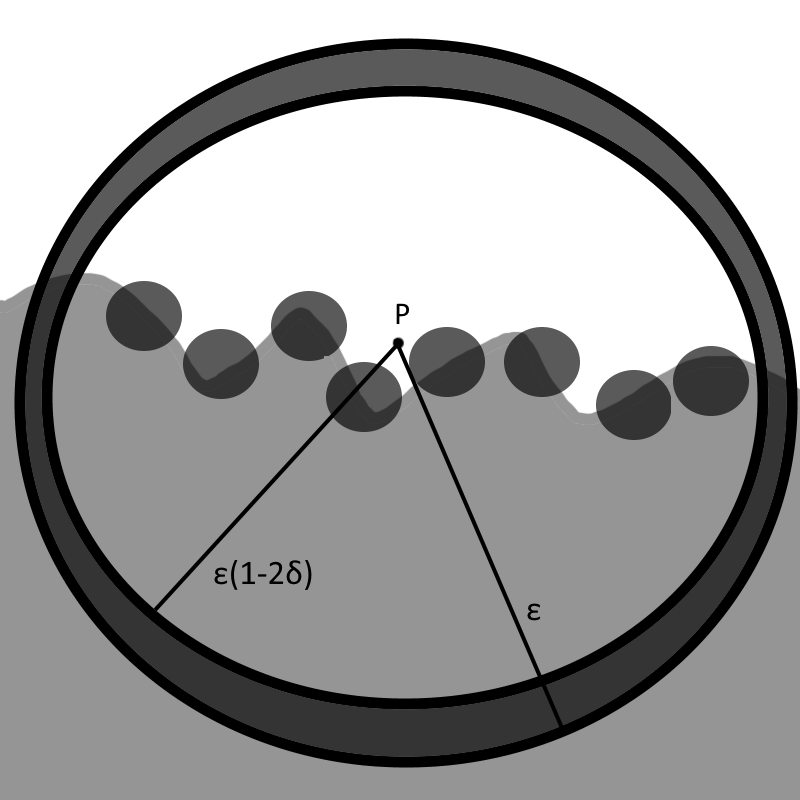
\includegraphics[width=0.4\textwidth]{covering lemma}
\end{figure}

If we write $F$ for the Radon-Nikod\'ym derivative of $\chi_\varepsilon$ with respect to the usual measure on $\Hyp^d$, then for every $x, z$ close to $O$ and $y \in B(z, \delta)$,
\begin{equation}\label{approximation of mollifier 2}
F(x - y) \sim \frac{1}{\varepsilon^d}\left(1 - \frac{d(x, Q)}{\varepsilon}\right)
\end{equation}
uniformly as $\delta, \varepsilon \to 0$.

Since $du$ is supported in $\bigcup_n 2V_n$,
$$|d\varphi|(x) - X\varphi(x) = \int_{B_\varepsilon} \chi_\varepsilon(x - \cdot)(|du| - Xu) \leq \sum_{n=0}^N \int_{2V_n} \chi_\varepsilon(x - \cdot)(|du| - Xu).$$
So, we shall show
\begin{equation}\label{bound on balls}
\int_{2V_n} \chi_\varepsilon(x - \cdot)(|du| - Xu) \lesssim_{g, p, P} \gamma^{O(1)} \int_{V_n} \chi_\varepsilon(x - \cdot)|du|
\end{equation}
for $n \geq 1$ and
\begin{equation}\label{bound on balls 2}
\int_{V_0} \chi_\varepsilon(x - \cdot)(|du| - Xu) \lesssim_{g, p, P} \gamma^{O(1)} \int_{B_\varepsilon} \chi_\varepsilon(x - \cdot)|du|,
\end{equation}
provided that $x = (r, \Theta)$ satisfies $r < \sigma$ and $\varphi \in (o(\gamma), 1 - o(\gamma))$.
If (\ref{bound on balls}, \ref{bound on balls 2}) are true, then since the balls $V_n$ are disjoint, we can sum over $n$ to obtain
\begin{equation}\label{claim on main mollifier lemma 2}|d\varphi|(x) - X\varphi(x) \lesssim_{g, p, P} \gamma^{O(1)} \int_{B_\varepsilon} \chi_\varepsilon(x - \cdot)|du| \leq \gamma^{O(1)} |d\varphi|(x),
\end{equation}
which implies (\ref{claim on main mollifier lemma}). Thus we may fix
$$x \in \partial^* U \cap \{r < \sigma\} \cap \{\varphi \in (f(\gamma), 1 - f(\gamma)),$$
and choose $\gamma$ so small that (\ref{claim on main mollifier lemma 2}) simplifies to $X\varphi(x) \gtrsim |d\varphi(x)|$.
Thus, in particular,
$$X\varphi(x) \gtrsim \int_{B_\varepsilon} \chi_\varepsilon(x - \cdot) |du| > 0.$$
By Lemma \ref{Giusti71}, $d\varphi$ is continuous, so the level sets of $\varphi$ must be $C^1$.
\end{proof}

\begin{proof}[Proof of (\ref{bound on balls})]
By (\ref{approximation of mollifier 2}), if $\gamma$ is small enough depending on $g$\footnote{One might worry that we frequently rescale $g$ in this paper.
However, in all of our rescalings, the curvature tensor remains in some bounded set, so these rescalings will never send $\gamma$ to $0$.}, then for every $y \in 2V_n$,
\begin{align*}
\int_{2V_n} \chi_\varepsilon(x - \cdot)(|du| - Xu) &\lesssim F_n(x) \int_{2V_n} |du| - Xu ~\vol, \\
F_n(x) &:= \frac{1}{\varepsilon^d}\left(1 - \frac{d(x, Q_n)}{\varepsilon}\right).
\end{align*}
If $\gamma$ is chosen small enough, then $\sigma > 2\delta\varepsilon$ and so if we set $W_n = B(Q_n, \sigma)$ and apply Proposition \ref{Monotonicity Formula},
\begin{align*}
\int_{2V_n}|du| - Xu ~\vol &\leq
B \left[\sigma^{1 - d}\int_{W_n} |du| - Xu ~\vol + \sigma^{1 - d}\int_{W_n} Xu ~\vol - (2\delta\varepsilon)^{1 - d}\int_{2V_n} Xu ~\vol \right],\\
B &:= e^{O(1)(\sigma^2 - 4\delta^2\varepsilon^2)}(2\delta\varepsilon)^{d - 1}.
\end{align*}
From Taylor's theorem and the fact that $\sigma > 2\delta\varepsilon$,
\begin{align*}
B \lesssim \delta^{d - 1} \varepsilon^{d - 1} + \sigma^2 \delta^{d - 1} \varepsilon^{d - 1} \lesssim \delta^{d - 1} \varepsilon^{d - 1}
\end{align*}
if $\gamma$ is small.
By (\ref{hypothesis on main mollifier lemma}),
$$\sigma^{1 - d}\int_{W_n} |du| - Xu ~\vol \leq \gamma^{\frac{1 - d}{2(d - 1)} + 1} = \gamma^{1/2}.$$
By Proposition \ref{Monotonicity Formula},
\begin{align*}
\sigma^{1 - d}\int_{W_n} Xu ~\vol - (2\delta\varepsilon)^{1 - d}\int_{2V_n} Xu ~\vol &\lesssim \sigma + (1 + \alpha)\sqrt{\sigma^{1 - d} \int_{W_n} |du| ~\vol - (2\delta\varepsilon)^{1 - d} \int_{2V_n} |du| ~\vol},\\
&\alpha := (d - 1)\log \frac{\sigma}{2\delta\varepsilon}.
\end{align*}

By Corollary \ref{scalar curvature monotonicity},
$$\sigma^{1 - d} \int_{W_n} X u ~\vol - (2\delta\varepsilon)^{1 - d} \int_{2V_n} |du| ~\vol \lesssim \sigma^2,$$
so by (\ref{hypothesis on main mollifier lemma}),
\begin{align*}
\sigma^{1 - d} \int_{W_n} |du| ~\vol - (2\delta\varepsilon)^{1 - d} \int_{2V_n} |du| ~\vol &= \sigma^{1 - d} \int_{W_n} |du| - Xu ~\vol \\
&\qquad + \sigma^{1 - d} \int_{W_n} Xu ~\vol - (2\delta\varepsilon)^{d - 1} \int_{W_n} |du| ~\vol \\
&\leq \gamma + O(\sigma^2) \lesssim \sigma^2.
\end{align*}
It follows from the definitions that
$$(1 + \alpha)\sigma \lesssim -\gamma^{1/2(d - 1)} \log \gamma \lesssim \gamma^{1/3(d - 1)}.$$
Summing up everything in this step of the proof thus far,
\begin{equation}\label{big bound 1}
\int_{2V_n} \chi_\varepsilon(x - \cdot)(|du| - Xu) ~\vol \lesssim \delta^{d - 1} \varepsilon^{d - 1} F_n(x) \gamma^{1/3(d - 1)}.
\end{equation}
Since $U$ has least perimeter, Proposition \ref{doubling dimension} implies that
$$\delta^{d - 1} \varepsilon^{d - 1} \lesssim \int_{V_n} |du| ~\vol,$$
so by (\ref{approximation of mollifier 2}, \ref{big bound 1}),
\begin{align*}
\int_{2V_n} \chi_\varepsilon(x - \cdot)(|du| - Xu) ~\vol
&\lesssim \gamma^{1/3(d - 1)} \int_{V_n} \chi_\varepsilon(x - \cdot)|du|.
\qedhere \end{align*}
\end{proof}

\begin{proof}[Proof of (\ref{bound on balls 2})]
From (\ref{approximation of mollifier 2}) it easily follows that for $y \in V_0$, $\chi_\varepsilon(x - y)/\vol(x - y) \lesssim \frac{\delta}{\varepsilon^d}$,
whence, by minimality of $\partial^* U$,
\begin{align*}
\int_{V_0} \chi_\varepsilon(x - \cdot)(|du| - Xu) &\lesssim \frac{\delta}{\varepsilon^d} \int_{B_\varepsilon} |du| ~\vol \lesssim \frac{\delta}{\varepsilon^d} |\partial B_\varepsilon| \lesssim \frac{\delta}{\varepsilon}.
\end{align*}
By Lemma \ref{Giusti71}, there exists $c > 0$ such that if $\varphi \in (c\gamma^2, 1 - c\gamma^2)$, then $d(x, \partial U) < \varepsilon(1 - \gamma)$, so in particular we can find $Q \in \partial^* U$ such that $d(x, Q) < \varepsilon(1 - \gamma)$.
If $d(y, Q) < \gamma\varepsilon/2$, then
$$d(x, y) \leq \varepsilon - \gamma\varepsilon + \frac{\gamma\varepsilon}{2} \leq \varepsilon - \frac{\gamma\varepsilon}{2},$$
so by (\ref{approximation of mollifier 2}), $\chi_\varepsilon(x - y)/\vol(x - y) \gtrsim \frac{\gamma}{\varepsilon^d}$
for every $y \in B(Q, \gamma\varepsilon/2)$.
In particular, since $\delta = \gamma^d$, minimality of $\partial^* U$ gives
\begin{align*}
\int_{V_0} \chi_\varepsilon(x - \cdot)(|du| - Xu) &\lesssim \frac{\delta}{\gamma^{d - 1}} \frac{\gamma^{d - 1}}{\varepsilon}\\
&\lesssim \gamma |\partial B(Q, \gamma\varepsilon/2)| \int_{B(Q, \gamma\varepsilon/2)} \chi_\varepsilon(x - \cdot) \\
&\lesssim \gamma \int_{B(Q, \gamma\varepsilon/2)} \chi_\varepsilon(x - \cdot) |du|\\
&\lesssim \gamma \int_{B_\varepsilon} \chi_\varepsilon(x - \cdot) |du|. \qedhere
\end{align*}
\end{proof}

%%%%%%%%%%%%%%%%%%%%%%%%%%%%%%%%%%%%%%%%%%%%%%%%%%%%%

\subsection{Proof of Lemma \ref{mollifier proposition}}
Select $t \in (0, 1)$ uniformly at random.
Let $w_n = (u_n)_{\gamma_n^4}$, let $c$ be the constant given by Lemma \ref{main mollifier lemma}, and let $a_n = c\gamma_n$, $b_n = 1 - c\gamma_n$.
0By Proposition \ref{Coarea2},
$$\int_{B_t} |dw_n| ~\vol = \int_0^1 |\partial^* \{w_n > y\} \cap B_t| ~dy \geq \int_{a_n}^{b_n} |\partial^* \{w_n > y\} \cap B_t| ~dy.$$
By the mean value theorem, there exists $y_n \in (a_n, b_n)$ such that
\begin{equation}\label{MVT mollifier}
|\partial^* \{w_n > y_n\} \cap B_t| \leq \frac{1}{b_n - a_n} \int_{B_t} |dw_n| ~\vol.
\end{equation}
If set $V_n = \{w_n > y_n\}$, $v_n = 1_{V_n}$, then $V_n$ has $C^1$ boundary in $B_t$ by definition of $a_n, b_n$, and from (\ref{claim on main mollifier lemma}), the locally uniform convergence (\ref{mollifier prop4}) holds.

So it remains to show that (\ref{mollifier prop1}--\ref{mollifier prop3}) hold almost surely.
Towards this end we will later show that
\begin{align}
|\partial V_n \cap B_t| &\leq |\partial^* U_n \cap B_t| + o(\gamma_n), \label{approximation of surface area} \\
\int_{\partial B_t} |u_n - v_n| ~\vol_{\partial B_t} &\lesssim \gamma_n^2. \label{approximation of volume}
\end{align}
If (\ref{approximation of surface area}, \ref{approximation of volume}) are true,
then by (\ref{a priori estimate 3}, \ref{approximation of volume}),
$$|\partial^* U_n \cap B_t| \leq |\partial V_n \cap B_t| + o(\gamma_n)$$
so by (\ref{approximation of surface area}), (\ref{mollifier prop2}) holds.
From an integration by parts using the estimate $1/2 \leq g(Y, Y) \leq 2$, and (\ref{approximation of volume}),
\begin{align*}
\left|\int_\Omega Y(u_j - v_j) ~\vol\right|
&\leq \left|\int_{\partial \Omega} (u_j - v_j)g(Y, \normal) ~\vol_{\partial \Omega}\right| \\
&\lesssim \int_{\partial \Omega} |u_j - v_j| ~\vol_{\partial \Omega} \lesssim \gamma_n^2
\end{align*}
which gives (\ref{mollifier prop3}).
By the fact that $U_n$ has least perimeter, and (\ref{a priori estimate 1}, \ref{mollifier prop2}),
\begin{align*}
|\partial V_n \cap B_t| &\leq |\partial U_n \cap B_t| + o(\gamma_n) \\
&= \eta(U_n, B_t) + o(\gamma_n)\\
&\leq \eta(V_n, B_t) + \int_{\partial B_t} |u_n - v_n| ~\vol_{\partial B_t} + o(\gamma_n),
\end{align*}
so by (\ref{approximation of volume}), (\ref{mollifier prop1}) holds.

%%%%%%%%%%%%%%%%%%%%%%%%%%%%%%%%%%%%%%%%%%%%%%%%%%%%%%%%%%%%%%%%

\begin{proof}[Proof of (\ref{approximation of surface area})]
By Lemma \ref{Giusti72}, one has
\begin{equation}\label{Giusti 720a}
\limsup_{n \to \infty} \int_{B_t} |du_n| - |dw_n| ~\vol \leq \limsup_{n \to \infty} \int_{B_{t + \gamma_n^4} \setminus B_t} |du_n| ~\vol.
\end{equation}
If we define $\mu = \sum_n \gamma_n|du_n| ~\vol$, then $\mu(B_1) < \infty$, since $(\gamma_n) \in \ell^1$ and $|\partial^* U_n \cap B_1|$ is uniformly bounded (c.f. Proposition \ref{doubling dimension}).
The hypotheses of \cite[(7.20)]{Giusti77} are (\ref{Giusti 720a}) and the fact that $\mu$ is a finite Borel measure on $B_1$, and the conclusion is that almost surely,
\begin{equation}\label{Giusti 720b}
\limsup_{n \to \infty} \gamma_n^{-2} \int_{B_t} |dw_n| - |du_n| ~\vol \leq 0.
\end{equation}
From (\ref{MVT mollifier}, \ref{Giusti 720b}), one has (\ref{approximation of surface area}).
\end{proof}

\begin{proof}[Proof of (\ref{approximation of volume})]
Let
$$f_n(t) = \gamma_n^{-4} \int_{B_t} |u_n - w_n| ~\vol.$$
By Lemma \ref{Giusti72} and the fact that $U_j$ has least perimeter in $B_1$,
$$\limsup_{n \to \infty} f_n(t) \leq \limsup_{n \to \infty} \int_{B_1} |du_n| ~\vol \leq |\partial B_1|.$$
Moreover, $f_n$ is monotone.
This implies that almost surely, $f_n'(t)$ is uniformly bounded in $n$.
But
$$f_n'(t) = \gamma_n^{-4} \int_{\partial B_t} |u_n - w_n| ~\vol_{\partial B_t},$$
so
\begin{equation}\label{mollify cubic gamma}
\int_{\partial B_t} |u_n - w_n| ~\vol_{\partial B_t} \lesssim \gamma_n^4.
\end{equation}
We now set $z_n = \min(y_n, 1 - y_n)$ and estimate
\begin{align*}
\int_{\partial B_t} |u_n - v_n| ~\vol_{\partial B_t} &= |\partial B_t \cap U_n \Delta V_n| \\
&= |\partial B_t \cap V_n \setminus U_n| + |\partial B_t \cap U_n \setminus V_n| \\
&\leq \frac{y_n}{z_n} |\partial B_t \cap V_n \setminus U_n| + \frac{1 - y_n}{z_n} |\partial B_t \cap U_n \setminus V_n|.
\end{align*}
From definition of $V_n$, $w_n - u_n > y_n$ on $V_n \setminus U_n$ and $u_n - w_n > 1 - y_n$ on $U_n \setminus V_n$, so
\begin{align*}
\int_{\partial B_t} |u_n - v_n| ~\vol_{\partial B_t} &\leq z_n^{-1} \int_{\partial B_t \cap U_n \setminus V_n} |u_n - w_n| ~\vol_{\partial B_t} + z_n^{-1}\int_{\partial B_t \cap V_n \setminus U_n} |u_n - w_n| ~\vol_{\partial B_t} \\
&\leq z_n^{-1} \int_{\partial B_t} |u_n - w_n| ~\vol_{\partial B_t}.
\end{align*}
But
$$z_n^{-1} \leq \max(y_n^{-1}, (1 - y_n)^{-1}) \leq \max(a_n^{-1}, b_n^{-1}) \lesssim \gamma_n^{-2}$$
whence
$$\int_{\partial B_t} |u_n - v_n| ~\vol_{\partial B_t} \lesssim \gamma_n^{-2} \int_{\partial B_t} |u_n - w_n| ~\vol_{\partial B_t},$$
so by (\ref{mollify cubic gamma}), (\ref{approximation of volume}) holds.
\end{proof}

\section{Regularity of minimal hypersurfaces}\label{DeGiorgiSection}
In this section we prove specialize to $\Hyp^d$ and show regularity of hypersurfaces, Theorem \ref{main lma}.

\begin{definition}
Let $u \in BV_\loc(\Hyp^d)$. The \dfn{approximate derivative} to $u$ at scale $n$ is the covector in $T_O' \Hyp^d$ defined by
$$\normal^{(n)}_\mu = \frac{\int_{B_{2^{-n}}} x \partial_\mu u ~\vol}{\int_{B_{2^{-n}}} |du| ~\vol}.$$
\end{definition}

Since $g(x\partial_\mu, x\partial_\nu) = \delta_{\mu\nu}$, $x\partial_\mu u = \normal_\mu|du|$.
Therefore, if $O$ is a Lebesgue point and $u = 1_U$, then $\normal^{(n)} \to \normal_U(O)$.

We can use the action of $\Iso(\Hyp^d)$ to define approximations to points $\normal_U(P)$, $P \in \Hyp^d$, as well.
To do this, let $A \in \Iso(\Hyp^d)$ map $O$ to $P$; then
$$\lim_{n \to \infty} (A^{-1})^* \normal^{(n)}(A^* u) = \normal_U(P)$$
if $P$ is a Lebesgue point of $A^* u$.
Actually, given a small open subset $\Omega$ of $\Hyp^d$, we can find a smooth family of isometries $A_P$ of $\Hyp^d$ parametrized by $P \in \Omega$ with $A_P(O) = P$.
It is clear that $(A^{-1})^* \normal^{(n)}(A^* u)$ depends continuously on $A$, and for almost every $P \in \Omega$, $P$ is a Lebesgue point.
So
$$\lim_{n \to \infty} (A_P^{-1})^* \normal^{(n)}(A_P^* u) = \normal_U(P)$$
is an almost-everywhere approximation of $\normal_U$ by a continuous $1$-form.
So our task is to show that $(\normal^{(n)})$ is a Cauchy sequence whose rate of convergence is unaffected by conjugation by isometries.

%%%%%%%%%%%%%%%%%%%%%%%%%%%%%%%%%%%%%%
\subsection{Representation as graphs}

We now show that $C^r$ hypersurfaces $N$ in $\Hyp^d$ can be represented as graphs of functions on $\RR_+ \times \RR^{d - 2}$ in a quantitative way.
This allows us to reduce the study of $N$ to the study of a weighted Plateau equation on $\RR_+ \times \RR^{d - 2}$.\footnote{One can identify $\RR_+ \times \RR^{d - 2}$ with $\Hyp^{d - 1}$, but we do \emph{not} do so here. Any balls, norms, et cetra, on $\RR_+ \times \RR^{d - 2}$ are meant in the euclidean sense.}
This result is a generalization of \cite[Theorem 4.8]{Giusti77}, and its proof is similar, but one needs to check that the integral curves are straight lines.

\begin{notation}
Let $\tilde B_r$ be the ball in $\RR_+ \times \RR^{d - 2}$ centered on $(1, 0, \dots, 0)$ of radius $r > 0$.
\end{notation}

\begin{lemma}\label{hopfKilling}
Let $N$ be a $C^r$ hypersurface in $\Hyp^d$ which bounds an open set, $r \in (0, 1)$, and
\begin{equation}\label{kappa-correct alignment}
||\normal_N^\sharp - x\partial_z||_{L^\infty(\tilde B_r \times \RR)} \leq \kappa^2
\end{equation}
where $\kappa \in [0, 1)$.
Then there exists a function $\omega \in C^r(\tilde B_r \to \RR)$
such that
\begin{align}
    N \cap (\tilde B_r \times \RR) &= \{(x, y, z) \in \tilde B_r\times \RR: z = \omega(x, y)\}, \label{N is a graph}\\
    ||d\omega||_{L^\infty(\tilde B_r)} &\leq \kappa. \label{derivative bounds}
\end{align}
\end{lemma}
\begin{proof}
We write $N = \partial U$, $u = 1_U$.
From the law of cosines and the fact that $\normal^\sharp$ and $x\partial_z$ both have unit length,
$$||\normal^\sharp - x\partial_z||_{L^\infty(N)}^2 = 2(1 - (\normal, x\partial_z)) = 2\left(1 - \frac{x\partial_z u}{|du|}\right).$$
Therefore
$$x\partial_z u \geq \left(1 - \frac{\kappa^2}{2}\right) |du|.$$
Given $\alpha$, a vector of unit length in $\RR_x \times \RR^{d - 2}_y \times (\RR_+)_z$, we can define a unit vector field
$$X_\alpha = \sum_\mu \alpha^\mu x\partial_\mu.$$
Then
$$\alpha^z x\partial_z u \geq \alpha^z \left(1 - \frac{\kappa^2}{2}\right) |du|$$
so from the Cauchy-Schwarz inequality and the fact that
$$1 - \left(1 - \frac{\kappa^2}{2}\right)^2 \leq \kappa^2,$$
we have
$$\left|\sum_{\mu \neq z} \alpha^\mu x\partial_\mu z\right| \leq \kappa\sqrt{1 - (\alpha^z)^2} |du|$$
and hence
\begin{equation}\label{hypothesis for Giusti47}
X_\alpha u \geq \left(\alpha^z - \frac{\alpha^z \kappa^2}{2} - \kappa\sqrt{1 - (\alpha^z)^2}\right)|du| \geq (\alpha^z - \kappa)|du|.
\end{equation}
Integrating $X_\alpha$ with initial conditions $P = (x_0, y_0, z_0) \in N$, we obtain the integral curve $(x(t), y(t), z(t))$,
\begin{align*}
x(t) &= x_0 e^{\alpha^x t}, \\
y_i(t) &= (y_0)_i + x_0 \frac{\alpha^{y_i}}{\alpha^x}(e^{\alpha^x t} - 1),\\
z(t) &= z_0 + x_0 \frac{\alpha^z}{\alpha^x}(e^{\alpha^x t} - 1)
\end{align*}
which extends to the line $\ell_\alpha = \{P + s\alpha: s \in \RR\}$ for $\alpha$ fixed.
By \cite[Remark 4.7]{Giusti77} and (\ref{hypothesis for Giusti47}), $N$ meets the cone $\bigcup_{\alpha^z > \kappa} \ell_\alpha$
only at $P$. This implies that $N$ is the graph of a function $\omega$, and
$$|\omega(x_2, y_2) - \omega(x_1, y_1)|^2 \leq \kappa^2 |x_2 - x_1|^2 + \kappa^2 |y_2 - y_1|^2$$
which gives (\ref{derivative bounds}).
\end{proof}

The hypothesis (\ref{kappa-correct alignment}) is important enough that we make the following definition which asserts the normal vector points in the $z$ direction \emph{on average} close to $O$.\footnote{It makes no sense to ask that the normal vector points in the $z$ direction at $O$, since $\normal^\sharp_U$ is just a measurable section and so may not be well-defined at $O$.}

\begin{definition}
A set $U$ of locally finite perimeter is \dfn{correctly aligned} at scale $n \in \ZZ$ if
$$(\normal^{(n)}_U)^\sharp = |\normal^{(n)}_U|\partial_z.$$
\end{definition}

Since we frequently will represent use Lemma \ref{hopfKilling} to replace $C^r$ hypersurfaces with graphs, we introduce the following notation.

\begin{notation}[hyperbolic space as a line bundle]\label{hyperbolic line bundle}
    If $\omega$ is a $C^r$ function $\Omega \to \RR_z$ with graph $N \subseteq \Hyp^d$, where $\Omega \subseteq (\RR_+)_x \times \RR^{d - 2}_y$ is open, we introduce the locally closed $C^r$ embedding
    \begin{align*}
        \Psi_N: \Omega &\to \Hyp^d \\
        (x, y) &\mapsto (x, y, \omega(x))
    \end{align*}
    which identifies $\Omega$ with $N$.
    We also introduce the projection
    \begin{align*}
        \Pi: \Hyp^d &\to (\RR_+)_x \times \RR^{d - 2}_y\\
        (x, y, z) &\mapsto (x, y)
    \end{align*}
    of which $\Psi_N$ is a section.
\end{notation}

Our next task is to show that $\omega$ solves a Plateau-type PDE if $N$ is a minimal hypersurface in $\Hyp^d$.
To that end, suppose that we are given a $d$-dimensional oriented real Hilbert space $(\Hilb, a)$, and an oriented basis $(\partial_0, \dots, \partial_{d - 1})$ which may not be orthonormal but which satisfies for every $i$
\begin{equation}\label{0th coordinate orthogonal}
a_{0i} = 0
\end{equation}
where $a_{\mu\nu} = a(\partial_\mu, \partial_\nu)$.
Here and in what follows Greek indices range over $0, \dots, d - 1$ while Latin indices range over $1, \dots, d - 1$\footnote{but $a$ is honestly an inner product, and not a Lorentz form}.

We write $a_{\hat 0 \hat 0}$ for the inner product on the span $\Hilb_0^\perp$ of $\partial_1, \dots, \partial_{d - 1}$ defined by $(a_{\hat 0 \hat 0})_{ij} = a_{ij}$.
We as usual write $a^{\mu\nu}$, $(a^{\hat 0 \hat 0})^{ij}$ for the components of the dual inner product, and $\delta_\mu^\nu$ for the components of the identity matrix.

\begin{definition}
The \dfn{Gramian matrix} of $v_1, \dots, v_{d - 1}$ is
$$\Gram(v_1, \dots, v_{d - 1})_{ij} = a(v_i, v_j).$$
The \dfn{cross product} $v_1 \times \cdots \times v_{d - 1}$ of vectors $v_1, \dots, v_{d - 1} \in \Hilb$ is defined to be the vector $v_0$
such that:
\begin{enumerate}
\item $a(v_0, v_i) = 0$,
\item $((-1)^{d - 1} v_0, v_1, \dots, v_{d - 1})$ is positively oriented, and
\item the length is
$$a(v_0, v_0) = |\det \Gram(v_1, \dots, v_{d - 1})|.$$
\end{enumerate}
\end{definition}

Here the orientation convention is chosen so that if $\partial_0, \dots, \partial_{d - 1}$ is an orthonormal basis, thus $a_{\mu\nu} = \delta_{\mu\nu}$, then the cross product is computed by the formal determinant
\begin{equation}\label{formal determinant}
v_1 \times \cdots \times v_{d - 1} = \begin{vmatrix}\partial_0 & \cdots & \partial_{d - 1} \\
v_1^0 & \cdots & v_1^{d - 1}\\
& \vdots \\
v_{d - 1}^0 & \cdots & v_{d - 1}^{d - 1}\end{vmatrix}
\end{equation}
which of course agrees with the orientation convention of the cross product on $\RR^3$.

\begin{lemma} \label{cross product formula}
Suppose that $\phi_1, \dots, \phi_{d - 1} \in \Hilb$ satisfy
\begin{equation}\label{cross product formula hypothesis}
\phi_i^\mu = \delta_i^\mu + \delta_0^\mu \psi_i
\end{equation}
for some $\psi \in (\Hilb_0^\perp)'$.
Let $h_{ij} = (a_{00})^{-1} a_{ij}$, and let $\normal \in \Hilb'$ be the unit covector which annihilates $\phi_1, \dots, \phi_{d - 1}$ with $((-1)^{d - 1}\normal^\sharp, \phi_1, \dots, \phi_{d - 1})$ positively oriented.
Then
\begin{align}
|\det \Gram(\phi_1, \dots, \phi_{d - 1})| &= (a_{00})^{d - 1} (1 + |\psi|_{h^{-1}}^2) \det h, \label{WeinsteinAronszajn} \\
(\phi_1 \times \cdots \times \phi_{d - 1})^\mu &= (a_{00})^{d/2} \sum_\nu a^{\mu \nu}(\delta_\nu^0 - \delta^i_\nu \psi_i) \sqrt{\det h}, \label{CrossProduct} \\
\normal_\mu &= \sqrt{\frac{g_{00}}{1 + |\psi|_{h^{-1}}^2}} (\delta^0_\mu - \delta^i_\mu \psi_i) \label{conormal crossproduct}.
\end{align}
\end{lemma}
\begin{proof}
In this proof, we use the Einstein convention.
We begin by computing
$$\Gram(\phi_1, \dots, \phi_{d - 1})_{ij} = a_{\mu \nu} \phi_i^\mu \phi_j^\nu = a_{00} \psi_i \psi_j + a_{ij}$$
which are the components of $a_{00}\psi \otimes \psi + a_{\hat 0 \hat 0} \in (\Hilb_0^\perp \otimes \Hilb_0^\perp)'$.
By the Weinstein-Aronszajn theorem \cite{Tao13}, $\det(1 + h^{-1}(\psi \otimes \psi)) = 1 + |\psi|_{h^{-1}}^2$, so
\begin{align*}
\det(a_{00}\psi \otimes \psi + g_{\hat 0 \hat 0})
&= (a_{00})^{d - 1} \det(\psi \otimes \psi + h) = (a_{00})^{d - 1} \det(h^{-1}(\psi \otimes \psi) + 1) \det h \\
&= (a_{00})^{d - 1} (1 + |\psi|_{h^{-1}}^2) \det h.
\end{align*}
Since $h$ is a quadratic form of signature $(+, \cdots, +)$, its determinant is positive and so (\ref{WeinsteinAronszajn}) holds.

We begin the proof of (\ref{CrossProduct}) by checking orthogonality:
\begin{align*}
a_{\mu\nu} a^{\mu \lambda} (\delta^0_\lambda - \delta^i_\lambda \psi_i)(\delta^\nu_0 \psi_i + \delta^\nu_i)
&= \delta^\lambda_\nu (\delta^0_\lambda - \delta^i_\lambda \psi_i)(\delta^\nu_0 \psi_i + \delta_i^\nu)
= \psi_i - \psi_i = 0.
\end{align*}
To check orientation we may assume that $a_{\mu\nu} = \delta_{\mu\nu}$ in which case we just need to check agreement with (\ref{formal determinant}):
$$\begin{vmatrix} \partial_0 && \cdots && \partial_{d - 1} \\
\psi_1 & 1 & 0 & \cdots & 0 \\
\psi_2 & 0 & 1 & \cdots & 0\\
&& \vdots \\
\psi_{d - 1} & 0 & \cdots & 0 & 1
\end{vmatrix} = \partial_0 - \sum_i \psi_i \partial_i.$$
To see that its length is $\det \Gram(\phi_1, \dots, \phi_{d - 1})$ we compute
\begin{align*}
a_{\mu \nu} a^{\mu \lambda}(\delta^0_\lambda - \delta^i_\lambda \psi_i) a^{\nu \kappa}(\delta_\kappa^0 - \delta_\kappa^j \psi_j)
&= (\delta_\mu^0 - \delta_\nu^i \psi_i)(a^{0 \nu} - a^{j \nu} \psi_j)\\
&= a^{00} - a^{0j} \psi_j - a^{0i} \psi_i + a^{ij} \psi_i \psi_j.
\end{align*}
Recalling (\ref{0th coordinate orthogonal}) we can rewrite this as
$$a_{\mu \nu} a^{\mu \lambda}(\delta^0_\lambda - \delta^i_\lambda \psi_i) a^{\nu \kappa}(\delta_\kappa^0 - \delta_\kappa^j \psi_j) = (a_{00})^{-1} + (a_{\hat 0 \hat 0})^{-1}(\psi \otimes \psi).$$
But $a_{00} (a_{\hat 0 \hat 0})^{-1} = h^{-1}$ so we deduce from (\ref{WeinsteinAronszajn})
$$a_{\mu \nu} a^{\mu \lambda}(\delta^0_\lambda - \delta^i_\lambda \psi_i) a^{\nu \kappa}(\delta_\kappa^0 - \delta_\kappa^j \psi_j) = (a_{00})^{-1} (1 + |\psi|_{h^{-1}}^2)
= \frac{|\det \Gram(\phi_1, \dots, \phi_{d - 1})|}{(a_{00})^d \det h}$$
which gives (\ref{CrossProduct}).
From (\ref{WeinsteinAronszajn}, \ref{CrossProduct}), (\ref{conormal crossproduct}) is immediate.
\end{proof}

Let $M$ be an open submanifold of $\Hyp^d = (\RR_+)_x \times \RR^{d - 2}_y \times \RR_z$ with the hyperbolic metric (\ref{hyperbolic metric}).
Let $\omega$ be a $C^1$ function on $M \cap (\RR_+ \times \RR^{d - 2})$, and write
$$N = \{(x, y, z) \in M: z = \omega(x, y)\}$$
for its graph in $M$.
Let $\partial_1, \dots, \partial_{d - 1}$ denote the coordinate vector fields on $\RR_+ \times \RR^{d - 2}$, and $\partial_0$ the coordinate vector field on $\RR_z$.
Then, in the language of Notation \ref{hyperbolic line bundle}, with $\Psi = \Psi_N$, $\psi = d\omega$, $\Hilb = T_{(x, y, \omega(x, y))} M$, $a = g|T_{(x, y, \omega(x, y))} M$, and $\phi_i = \Psi_* \partial_i$, we have (\ref{cross product formula hypothesis}).
In particular, $\phi_1, \dots, \phi_{d - 1}$ span $T_{(x, y, \omega(x, y))}N$.
We also have
$$h_{ij} = x^2 g_{ij} = x^2 x^{-2} \delta_{ij} = \delta_{ij}.$$
So by Lemma \ref{cross product formula}, the conormal $\normal$ to $N$ at $(x, y, \omega(x, y))$ is given by
$$(\Psi^* \normal)_\mu = \sqrt{\frac{x}{1 + |d\omega|^2}} (\delta_\mu^0 - \delta_\mu^i \omega_{,i})$$
where $|\cdot|$ is the euclidean length.
If we denote $\slashed g_{ij} = g(\phi_i, \phi_j)$, then
$$\slashed g = \Gram(\phi_1, \dots, \phi_{d - 1})$$
and so the volume form on $N$ is given by
$$\Psi^* \vol_N = x^{1 - d} \sqrt{1 + |d\omega|^2} ~dx dy.$$
Therefore we introduce:

\begin{definition}
    The \dfn{hyperbolic Plateau energy} of a $1$-form $\psi$ on $(\RR_+)_x \times \RR^{d - 2}_y$ is the $d-1$-form
    $$\Lagrange(\psi) = x^{1 - d} \sqrt{1 + |\psi|^2} ~dxdy$$
    where the metric is euclidean.
\end{definition}

We now have
\begin{equation}\label{Lagrangian formula}
    \Psi_N^* \vol_N = \Lagrange(d\omega)
\end{equation}
if $N$ is the graph of $\omega \in C^1(\Omega)$, $\Omega \subseteq \RR_+ \times \RR^{d - 2}$.
If $\normal$ denotes the conormal $1$-form then we have
\begin{equation}\label{Lagrangian normal z}
(\Psi^*_N \normal)_z \Lagrange(d\omega) = x^p ~dxdy
\end{equation}
where $p = 3/2 - d$, and
\begin{equation}\label{Lagrangian normal xy}
(\Psi^*_N \normal)_i \Lagrange(d\omega) = x^p \partial_i \omega(x, y) ~dxdy
\end{equation}
whenever $i \in \{x, y_1, \dots, y_{d - 2}\}$.

If $N$ is a minimal hypersurface, then $d\omega$ is a minimizer of $\Lagrange(d\omega)$, and in particular solves the Plateau-type PDE
\begin{equation}\label{Plateau PDE}
    \Div \frac{\grad \omega}{\sqrt{1 + |\grad \omega|^2}} + \frac{1 - d}{x^d \sqrt{1 + |\grad \omega|^2}} \partial_x \omega = 0,
\end{equation}
though we will seldom use this PDE directly.

%%%%%%%%%%%%%%%%%%%%%%%%%%%%%%%%%%%%%

\subsection{Excess versus Plateau energy}
In this subsection we introduce the \dfn{excess} of a set $U$ of locally finite perimeter, which roughly speaking determines how much the normal vector to $U$ can twist in a neighborhood of $O$.
We then show that the excess controls the modulus of continuity of the normal vector and in turn is controlled by the Plateau energy.
Notions of excess for $\RR^d$ appear in the monographs of Federer \cite[\S5.3.1]{federer2014geometric} and Giusti \cite[Chapter 6]{Giusti77}.

We begin by showing that on average, the errors incurred by the hyperbolic metric are negligible.
In fact, we will always be able to disregard terms of order $4^{-n}$, so our next few lemmata allow us to ignore

\begin{notation}
We identify $m$-forms on $\RR_+ \times \RR^{d - 2}$ with smooth maps $\RR_+ \times \RR^{d - 2} \to (\RR^{d - 1})^{\wedge m}$.
We identify vectors in $(\RR^{d - 1})^{\wedge m}$ with constant $m$-forms, and for a $m$-form $\psi$ define the constant $m$-form
$$(A_n \psi)_I = \dashint_{\tilde B_{2^{-n}}} \psi_I(x, y) ~dxdy$$
where $I$ ranges over ascending $m$-multiindices.
\end{notation}

\begin{lemma}\label{ball difference is harmless}
The symmetric difference of balls has measure
$$|\Pi(B_{2^{-n}}) \Delta \tilde B_{2^{-n}}| \lesssim 2^{-nd}.$$
In particular, if $\psi$ is a $m$-form then
$$(A_n \psi)_I = \dashint_{\tilde B_{2^{-n}}} \psi_I(x, y) ~dxdy + O(2^{-n}).$$
\end{lemma}
\begin{proof}
TODO. It's true if $d = 2$ at least. We need to rewrite a lot of the rest of the proof to use $\tilde B$ instead of $\Pi B$.
\end{proof}

\begin{lemma}\label{average of xp is harmless}
For every $p \in \RR$ one has
$$A_n(x^p) = 1 + O(4^{-n})$$
where the implied constant depends on $p$.
\end{lemma}
\begin{proof}
TODO: Simplify this by using $\tilde B$
According to (\ref{sup in a ball}), we can find a minimal rectangle $I \Subset \RR^{d - 2}$ such that
$$\Pi(B_{2^{-n}}) \subseteq (\exp(-2^{-n}), \exp(2^{-n})) \times I,$$
so by Fubini's theorem,
\begin{align*}|A_n(x^p - 1)| &= \left|\dashint_{\Pi(B_{2^{-n}})} (x^p - 1) ~dxdy\right| \lesssim \frac{|I|}{|\Pi(B_{2^{-n}})|} \left|\int_{\exp(-2^{-n})}^{\exp(2^{-n})} (x^p - 1)~ dx\right|;
\end{align*}
from minimality we have $|I| \lesssim 2^{n + 1} |\Pi(B_{2^{-n}})|$.
Making the substitution $\tilde x = \log x$ and disposing of the Jacobian as $1/2 \leq e^{\tilde x} \leq 2$, we obtain
$$|A_n(x^p - 1)| \lesssim \left|\dashint_{-2^{-n}}^{2^{-n}} (e^{p\tilde x} - 1) ~d\tilde x\right|.$$
From Taylor's theorem and the parity of $\tilde x$,
\begin{align*}
|A_n(x^p - 1)| &\lesssim \left|\dashint_{-2^{-n}}^{2^{-n}} \tilde x + O(\tilde x^2) ~d\tilde x\right| \\
&\lesssim 2^n \int_0^{2^{-n}} \tilde x^2 ~d\tilde x \lesssim 2^n 8^{-n} = 4^{-n}. \qedhere
\end{align*}
\end{proof}

\begin{lemma}\label{normal has length 1}
Let $\normal^{(n)}$ be the approximate derivative of $1_U$ where $U$ is a set of locally finite perimeter.
$$|\normal^{(n)}| \leq 1 + O(4^{-n}).$$
\end{lemma}
\begin{proof}
Let $\kappa > 0$ be a parameter to be chosen.
We may assume that $U$ is correctly aligned, and under that assumption, Proposition \ref{mollifier quant} furnishes a set $V$ of $C^1$ perimeter in $B_{2^{-n}}$ such that, with $u = 1_U$, $v = 1_V$,
\begin{align*}
\max\left[\left|\int_{B_{2^{-n}}} |du| - |dv| ~\vol\right|, \max_\mu \left|\int_{B_{2^{-n}}} x\partial_\mu(u - v) ~\vol\right|\right] &\leq 8^{-n} \int_{B_{2^{-n}}} |du| ~\vol, \\
||\normal^\sharp_V - x\partial_z||_{L^\infty(B_{2^{-n}})} &\leq 64^{-n}.
\end{align*}
(TODO: Taking the limit $t \to 0$)
We now show that it is harmless to replace $U$ with $V$. In fact
\begin{align*}
|\normal^{(n)}_\mu(u) - \normal^{(n)}_\mu(v)|
&= \left|\frac{\int_{B_{2^{-n}}} x\partial_\mu u ~\vol}{\int_{B_{2^{-n}}} |du| ~\vol} - \frac{B_{2^{-n}} x\partial_\mu v}{\int_{B_{2^{-n}}} |dv| ~\vol}\right|\\
&= \left[\int_{B_{2^{-n}}} |du| ~\vol \int_{B_{2^{-n}}} |dv| ~\vol\right]^{-1} \\
&\qquad \left[\left|\int_{B_{2^{-n}}} |du| - |dv| ~\vol\right| \int_{B_{2^{-n}}} x\partial_\mu u ~\vol+ \int_{B_{2^{-n}}} |du| ~\vol \left|\int_{B_{2^{-n}}} x\partial_\mu(u - v) ~\vol\right|\right] \\
&\lesssim 8^{-n}.
\end{align*}
So, without loss of generality, $\partial U$ is a $C^1$ hypersurface which satisfies
$$||\normal^\sharp - x\partial_z||_{L^\infty(B_{2^{-n}})} \leq 64^{-n}.$$
Therefore by Lemma \ref{hopfKilling}, the fact that $(dx, dy_1, \dots, dy_{d-2}, dz)$ is an orthonormal basis of $T'_O\Hyp^d$, and (\ref{Lagrangian normal z}, \ref{Lagrangian normal xy}) there is a $C^1$ function $\omega$ such that $||d\omega||_{L^\infty} \leq 8^{-n}$ and
$$|\normal^{(n)}|^2 = \frac{1}{|\partial U \cap B_{2^{-n}}|} \left[\left(\int_{\Pi(B_{2^{-n}})} x^p ~dxdy\right)^2 + \sum_i \left(\int_{\Pi(B_{2^{-n}})} x^p \partial_i \omega(x, y) ~dxdy\right)^2\right].$$
The estimate on $d\omega$ implies that
$$|\normal^{(n)}|^2 = \frac{1 + O(8^{-n})}{|\partial U \cap B_{2^{-n}}|}\left(\int_{\Pi(B_{2^{-n}})} x^p ~dxdy\right)^2$$
and now the claim follows easily from the fact that
$$|\Pi(B_{2^{-n}})| \leq |\partial U \cap B_{2^{-n}}|$$
and Lemmata \ref{ball difference is harmless}, \ref{average of xp is harmless}.
\end{proof}

\begin{definition}
The \dfn{excess} of a set $U$ of locally finite perimeter at scale $n$ is
$$\Exc_n(U) = 2^{n(d - 1)} (1 - |\normal^{(n)}|) \int_{B_{2^{-n}}} |d1_U| ~\vol.$$
\end{definition}

The first basic property of the excess is rotation-invariance, which we now formulate.

\begin{notation}
We define an action
\begin{equation}\label{hyperbolic rotation}
    \Phi: \Orth(\RR^d) \to \Iso(\Hyp^d)
\end{equation}
of the orthogonal group $\Orth(\RR^d)$, as well as the representation
\begin{align*}
\Orth(\RR^d) &\to \GL(BV_\loc(\RR^d))\\
A^* u(P) &:= u(\Phi(A)(P))
\end{align*}
of $\Orth(\RR^d)$ on $BV_\loc(\RR^d)$, as follows.
Recall that the hyperbolic metric in the ball model $\DD^d$ is radial, so the natural action of the orthogonal group $\Orth(\RR^d)$ on $\DD^d$ is by isometry, and if we use the Cayley transform to identify the origin of $\DD^d$ with $O$, then we obtain a faithful action (\ref{hyperbolic rotation}) whose orbits are the spheres $\partial B_r$ centered on $O$.
\end{notation}

\begin{lemma}\label{excess rotation invariant}
For every $A \in \Orth(\RR^d)$ and $u \in BV_\loc(\Hyp^d)$,
$$\Exc_n(A^* u) = \Exc_n(u).$$
\end{lemma}
\begin{proof}
Since $A$ is an isometry, $|(d A^* u)_{\Phi(A)(P)}| = |(du)_P|$, so
\begin{align*}
\int_{B_{2^{-n}}} |dA^*u| ~\vol &= \int_0^{2^{-n}} \int_{\partial B_r} |dA^* u| ~\vol_{\partial B_r} ~dr = \int_0^{2^{-n}} \int_{\partial B_r} |du| ~\vol_{\partial B_r} ~dr\\
&= \int_{B_{2^{-n}}} |du| ~\vol
\end{align*}
since $(A^{-1})^* \vol_{\partial B_r} = \vol_{\partial B_r}$.
Since $A$ is an isometry, $|A_* (x \partial_\mu)| = 1$ and $(A_*(x \partial_\mu))_\mu$ is an orthonormal basis of $T_O \Hyp^d$.
The claim follows.
\end{proof}

We now show that the rate of convergence of the approximate derivative is given by the excess.
An analogous estimate for the euclidean case is due to Miranda \cite[pg661]{Miranda66}; our contribution is to deal with the correction terms that arise from the hyperbolic metric.

\begin{lemma} \label{excess bounds Cauchy sequence}
Let $U$ be a set of locally finite perimeter.
Let $\normal^{(n)}$ be the approximate derivative of $1_U$ and suppose that $n$ is larger than some absolute constant. Then
$$|\normal^{(n)} - \normal^{(n + m)}|^2 \leq \frac{2^{3 + n(1 - d)}}{\int_{B_{2^{-(n + m)}}} |du| ~\vol} \Exc_n(u) + O(2^{m(d - 1) - 2n}).$$
\end{lemma}
\begin{proof}
From the law of cosines and Lemma \ref{normal has length 1},
\begin{align*}
|\normal^{(n)} - \normal^{(n + m)}|^2 &= |\normal^{(n)}|^2 + |\normal^{(n + m)}|^2 - 2 g(\normal^{(n)}, \normal^{(n + m)})\\
&\leq 2(1 - g(\normal^{(n)}, \normal^{(n + m)}) + O(16^{-n})) \\
&= \frac{2}{\int_{B_{2^{-(n + m)}}} |du| ~\vol} \int_{B_{2^{-(n + m)}}} (1 + O(16^{-n}))|du| - \sum_\mu x \partial_\mu u \normal_\mu^{(n)} ~\vol.
\end{align*}
Applying Lemma \ref{normal has length 1} alongside the Cauchy-Schwarz inequality,
$$\sum_\mu x \partial_\mu u \normal_\mu^{(n)} \leq |du|(1 + O(4^{-n}))$$
so
\begin{align*}
|\normal^{(n)} - \normal^{(n + m)}|^2 &\leq \frac{2}{\int_{B_{2^{-(n + m)}}} |du| ~\vol} \int_{B_{2^{-n}}} (1 + O(4^{-n}))|du| - \sum_\mu x \partial_\mu u \normal_\mu^{(n)} ~\vol\\
&= \frac{2}{\int_{B_{2^{-(n + m)}}} |du| ~\vol} (1 + O(4^{-n}) - |\normal^{(n)}|^2) \int_{B_{2^{-n}}} |du| ~\vol.
\end{align*}
The claim now follows from the inequality $1 - a^2 \leq 1 - 2a$ valid for $a < 2$ (and in particular for $a = |\normal^{(n)}|^2$ if $n$ is large).
\end{proof}

We now show that the excess is controlled by the Plateau energy.
In the euclidean case, this result is not an approximation but an equality (c.f. \cite[pg83]{Giusti77}), and so in that case the proof of the following lemma is trivial.

\begin{lemma}\label{excess vs plateau energy}
Let $\omega \in C^1(\Omega)$ satisfy $||d\omega||_{L^\infty} \lesssim 1$. Then
\begin{align*}
    \Exc_n(1_{\omega(x, y) < z}) = 2^{n(d - 1)} \left[\int_{\Pi(B_{2^{-n}})} \Lagrange(d\omega) - \Lagrange(A_n d\omega)\right] + O(4^{-n}).
\end{align*}
\end{lemma}
\begin{proof}
Let $u(x, y, z) = 1_{\omega(x, y) < z}$, let $N$ be the graph of $\omega$, and let $\normal^{(n)}$ be the approximate derivative of $u$.
It follows from the definitions, the fact that $|du|$ is the Radon-Nikod\'ym derivative $\vol_N/\vol$, and (\ref{Lagrangian formula}), that
$$\normal^{(n)}_\mu \int_{B_{2^{-n}}} |du| ~\vol = \int_{B_{2^{-n}}} \normal_\mu |du| ~\vol = \int_{B_{2^{-n}} \cap N} \normal_\mu \vol_N = \int_{\Pi(B_{2^{-n}})} (\Psi_N^* \normal)_\mu \Lagrange(d\omega).$$
We apply Lemma \ref{ball difference is harmless} to deduce
$$\normal^{(n)}_\mu \int_{B_{2^{-n}}} |du| ~\vol = \int_{\tilde B_{2^{-n}}} (\Psi_N^* \normal)_\mu \Lagrange(d\omega) + O(2^{-nd}).$$
From the fact that $(dx, dy_1, \dots, dy_{d - 2}, dz)$ is an orthonormal basis of $T_O' \Hyp^d$, it follows that
$$|\normal^{(n)}|^2 \left(\int_{B_{2^{-n}}} |du| ~\vol\right)^2 = \sum_\mu \left(\int_{\Pi(B_{2^{-n}})} (\Psi_N^* \normal)_\mu \Lagrange(d\omega)\right)^2 + O(2^{(1 - 2d)n})$$
so from (\ref{Lagrangian normal z}, \ref{Lagrangian normal xy}),
\begin{align*}
    |\normal^{(n)}|^2 \left(\int_{B_{2^{-n}}} |du| ~\vol\right)^2 &= \left(\int_{\Pi(B_{2^{-n}})} x^p ~dxdy\right)^2 + \sum_i \left(\int_{\Pi(B_{2^{-n}})} x^p \partial_i \omega(x, y) ~dxdy \right)^2 \\
    &= |\Pi(B_{2^{-n}})|^2 |A_n (x^p)|^2 \left(1 + \frac{|A_n(x^p d\omega)|^2}{|A_n (x^p)|^2}\right) + O(2^{(1 - 2d)n}).
\end{align*}
Using Lemma \ref{average of xp is harmless} and Taylor's theorem,
\begin{align*}
    |A_n(x^p d\omega) - A_n (d\omega)| &\leq ||d\omega||_{L^\infty} |A_n (x^p - 1)| \lesssim 4^{-n}
\end{align*}
and so by Proposition \ref{doubling dimension},
$$|\normal^{(n)}| \int_{B_{2^{-n}}} |du| ~\vol = |\Pi(B_{2^{-n}})| \sqrt{1 + |A_n d\omega|^2} + O(2^{-n(d + 1)}).$$
We rewrite
$$|\Pi(B_{2^{-n}})| \sqrt{1 + |A_n d\omega|^2} = \int_{\Pi(B_{2^{-n}})} \Lagrange(A_nd\omega) + \int_{\Pi(B_{2^{-n}})} (1 - x^{1 - d})\sqrt{1 + |A_n d\omega|^2} ~dxdy$$
and bound the remainder term using Lemma \ref{average of xp is harmless} and Proposition \ref{doubling dimension}:
$$0 \leq \int_{\Pi(B_{2^{-n}})} (1 - x^{1 - d})\sqrt{1 + |A_n d\omega|^2} ~dxdy \lesssim \int_{\Pi(B_{2^{-n}})} (1 - x^{1-d}) ~dxdy \lesssim O(2^{-n(d + 1)}).$$
The claim now follows from the definition of the excess.
\end{proof}

%%%%%%%%%%%%%%%%%%%%%%%%%%%%%%%%%%
\subsection{Plateau versus Dirichlet}

Here we compare the Plateau energy to the Dirichlet energy, and apply potential theory to get a multiplicative gain when we pass from a scale $n$ to its successor $n + 1$.
Such a strategy was classically employed by Miranda \cite[Teorema 4.3]{Miranda66} to show the regularity of minimal hypersurfaces in $\RR^d$.
To see why one should expect it to work, even in the hyperbolic case, let $\omega \in C^1$, and note that (\ref{derivative bounds}) gives a sufficient condition for $|d\omega|$ to be small in a neighborhood of $x = 1, y = 0$.
But the linearization of Plateau's equation (\ref{Plateau PDE}) at $x = 1, y = 0, |d\omega| = 0$ is the Laplace equation $\Delta \omega = 0$, so $\omega$ is well-approximated by harmonic functions.
The desired gain holds for harmonic functions (\ref{Miranda41}) and so should at least approximately hold for the minimal surfaces.\footnote{The generalization of (\ref{Plateau PDE}) to arbitrary Riemannian manifolds linearizes to an elliptic PDE of second order, and it would be interesting to show that such PDE also satisfy an analogue of (\ref{Miranda41}), but we do not attempt this here.}

We turn to the details.
Let
$$\DirL(\psi) = \frac{|\psi|^2}{2} ~dxdy$$
be the Dirichlet energy of a $1$-form $\psi = d\omega$ on $(\RR_+)_x \times \RR^{d - 2}_y$.
In the below computation we suppress the $dxdy$.
Given $1$-forms $\psi_1, \psi_2$, there exists $\xi \in [|\psi_1|, |\psi_2|]$ such that
\begin{equation}\label{Taylor remainder Dirichlet}
\Lagrange(\psi_1) - \Lagrange(\psi_2) = x^{1 - d}\left(\frac{|\psi_1|^2 - |\psi_2|^2}{2\sqrt{1 + |\psi_2|^2}} - \frac{(|\psi_1|^2 - |\psi_2|^2)^2}{8(1 + \xi^2)^{3/2}}\right).
\end{equation}
The second term of (\ref{Taylor remainder Dirichlet}) is negative and $\sqrt{1 + |\psi_2|^2} \geq 1$, so it follows that
\begin{equation}\label{Taylor lower bound}
\Lagrange(\psi_1) - \Lagrange(\psi_2) \leq x^{1 - d} (\DirL(\psi_1) - \DirL(\psi_2)).
\end{equation}
If in addition $||\psi_2||_{L^\infty} \leq 1$, then
$$4\sqrt{1 + |\psi_2|^2} \leq 8 \leq 8(1 + \xi^2)^{3/2}$$
so we conclude
\begin{equation}\label{Taylor upper bound}
\Lagrange(\psi_1) - \Lagrange(\psi_2) \geq \frac{x^{1 - d}}{\sqrt{1 + |\psi_2|^2}} (\DirL(\psi_1) - \DirL(\psi_2) - (\DirL(\psi_1) - \DirL(\psi_2))^2).
\end{equation}
For every harmonic function $h$, by \cite[Lemma 4.1]{Miranda66},
\begin{equation}\label{Miranda41}
\int_{\tilde B_{2^{-(n+1)}}} \DirL(dh) - \DirL(A_n dh) \leq 2^{-(d + 1)} \int_{\tilde B_{2^{-n}}} \DirL(dh) - \DirL(A_n dh).
\end{equation}
Moreover, the mean-value property of $dh$ implies that for every $1$-form $\psi$,
\begin{equation}\label{MVP derivative}
\int_{\tilde B_{2^{-n}}} \DirL(dh - \psi) = \int_{\tilde B_{2^{-n}}} \DirL(dh) - \DirL(\psi).
\end{equation}

On first reading of the below lemma, the reader may take $c = 10^{-3}$, $O(c) = 10^{-1}$ and $n^* = 10$; in fact, $c$ will later be chosen to be a dimensional constant.
Roughly speaking, one should think of $\beta$ as comparable to $2^{-(n - n^*)}$, and $\kappa$ as the ``error incurred by mollification".

\begin{lemma}\label{DGL1}
For every $c > 0$ there exists a scale $n^* \in \ZZ$ with the following property:

Let $\omega \in C^1(\Omega)$, suppose that $\kappa, \beta \in (0, 1)$ and $n \geq n^*$ satisfy
\begin{align}
||d\omega||_{L^\infty(\tilde B_{2^{-n}})} &\leq \kappa, \label{DGL1 1}\\
\int_{\tilde B_{2^{-n}}} \Lagrange(d\omega) - \Lagrange(A_n d\omega) &\leq \beta, \label{DGL1 2}\\
\int_{\tilde B_{2^{-n}}} \Lagrange(d\omega) &\leq \eta(\{(x, y, z) \in \Hyp^d: z < \omega(x, y)\}, 2^{-n}) + \beta \kappa. \label{DGL1 3}
\end{align}
Then
$$\int_{\tilde B_{2^{-(n + 1)}}}\Lagrange(d\omega) - \Lagrange(A_{n + 1} d\omega) \leq (1 + O(c)) 2^{-(d + 1)} \beta + O(\beta \sqrt \kappa)$$
where all constants only depend on $d$.
\end{lemma}
\begin{proof}
Choose $n^*$ so large that
\begin{equation}\label{x to c}
1 - c \leq \inf_{(x, y) \in \tilde B_{2^{-n^*}}} x^{1 - d} < \sup_{(x, y) \in \tilde B_{2^{-n^*}}} x^{1 - d} \leq 1 + c
\end{equation}
and suppose that $n \geq n^*$.
Let $h$ be the harmonic function on $\tilde B_{2^{-n}}$ such that
\begin{equation}\label{trace equation}
h = \omega \text{ on } \partial \tilde B_{2^{-n}}.
\end{equation}
By definition of $\eta$ and (\ref{DGL1 3}),
\begin{align*}
\int_{\tilde B_{2^{-(n + 1)}}} \Lagrange(d\omega) - \Lagrange(dh)
&\leq \int_{\tilde B_{2^{-n}}} \Lagrange(d\omega) - \eta(\{(x, y, z) \in \Hyp^d: z < \omega(x, y)\}, 2^{-n}).
\end{align*}
Therefore
\begin{equation}\label{bound on domega - dh}
\int_{\tilde B_{2^{-(n + 1)}}} \Lagrange(d\omega) - \Lagrange(dh) \leq \beta\kappa.
\end{equation}

The rest of the proof is essentially identical to \cite[Lemma 4.2]{Miranda66}, but as this is a crucial step, we include it for completeness.
By (\ref{Taylor lower bound}, \ref{x to c}),
$$\int_{\tilde B_{2^{-(n + 1)}}} \Lagrange(d\omega) - \Lagrange(A_{n + 1}d\omega) \leq (1 + c)\int_{\tilde B_{2^{-(n + 1)}}} \DirL(d\omega) - \DirL(A_{n + 1}d\omega).$$
Since $A_{n + 1}d\omega$ is the mean of $d\omega$, for every $\varepsilon \in (0, 1)$,
\begin{align*}
\int_{\tilde B_{2^{-(n + 1)}}} \DirL(d\omega) - \DirL(A_{n + 1}d\omega)
&\leq \int_{\tilde B_{2^{-(n + 1)}}} \DirL(d\omega - A_nd\omega) \\
&\leq (1 + \varepsilon^{-1}) \int_{\tilde B_{2^{-(n + 1)}}} \DirL(d(\omega - h)) \\
&\qquad +(1 + \varepsilon) \int_{\tilde B_{2^{-(n + 1)}}} \DirL(dh - A_nd\omega) \\
&=: O(\varepsilon^{-1}) I + (1 + \varepsilon) J.
\end{align*}
From the positivity of Dirichlet energy and (\ref{MVP derivative}, \ref{Taylor upper bound}),
\begin{align*}
I &\leq \int_{\tilde B_{2^{-n}}} \DirL(d(\omega - h)) = \int_{\tilde B_{2^{-n}}} \DirL(d\omega) - \DirL(dh) \lesssim \int_{\tilde B_{2^{-n}}} \Lagrange(d\omega) - \Lagrange(dh)
\end{align*}
so by (\ref{bound on domega - dh}),
\begin{equation}\label{bound on I}
I \lesssim \beta\kappa.
\end{equation}
Moreover, by (\ref{MVP derivative}),
$$J = \int_{\tilde B_{2^{-(n + 1)}}} \DirL(dh) - \DirL(A_nd\omega).$$
From (\ref{trace equation}) and Stokes' theorem, there are constants $C_m > 0$ such that
$$A_m d\omega = C_m \int_{\partial \tilde B_{2^{-m}}} \omega ~dS = C_m \int_{\partial \tilde B_{2^{-m}}} h ~dS = A_m dh$$
which along with (\ref{Miranda41}, \ref{MVP derivative}) implies that
$$J \leq 2^{-(d + 1)} \int_{\tilde B_{2^{-n}}} \DirL(dh) - \DirL(A_nd\omega) = 2^{-(d + 1)} \int_{\tilde B_{2^{-n}}} \DirL(dh - A_n d\omega).$$
We further estimate, using (\ref{bound on I}),
\begin{align*}
J &\leq (1 + \varepsilon) 2^{-(d + 1)} \int_{\tilde B_{2^{-n}}} \DirL(d\omega - A_n d\omega) + O(\varepsilon^{-1} I) \\
&:= (1 + \varepsilon) 2^{-(d + 1)} K + O(\varepsilon^{-1} \beta \kappa).
\end{align*}
To estimate $K$ we apply (\ref{MVP derivative}, \ref{x to c}, \ref{Taylor upper bound}) to obtain
\begin{align*}
K &= \int_{\tilde B_{2^{-n}}} \DirL(d\omega) - \DirL(A_n d\omega) \\
&\leq (1 + O(c)) \int_{\tilde B_{2^{-n}}} \Lagrange(d\omega) - \Lagrange(A_n d\omega) + O(1) \int_{\tilde B_{2^{-n}}} (\DirL(d\omega) - \DirL(A_n d\omega))^2.
\end{align*}
From (\ref{DGL1 1}, \ref{DGL1 2}), it follows that
\begin{align*}
K &\leq (1 + O(c))\beta + O(||d\omega||_{L^\infty(\tilde B_{2^{-n^*}})}) \int_{\tilde B_{2^{-n}}} \DirL(d\omega) - \DirL(A_n d\omega)\\
&\leq \beta(1 + O(c + \kappa)).
\end{align*}
If we set $\varepsilon = \sqrt \kappa$ then it follows that
\begin{align*}
\int_{\tilde B_{2^{-(n+1)}}} \DirL(d\omega) - \DirL(A_n d\omega) &\leq (1 + O(c)) 2^{-(d + 1)} \beta + O(\beta \sqrt \kappa). \qedhere
\end{align*}
\end{proof}

%%%%%%%%%%%%%%%%%%%%%%%%%%%%%%%%%%%%%%%%%%%%%%%%%

\subsection{de Giorgi lemma}
The classical de Giorgi lemma \cite{deGiorgi61} transfers the multiplicative gains of Lemma \ref{DGL1} to the excess of a set of least perimeter.
Iterating it allows us then to deduce the regularity of the reduced boundary.
For our analogue on $\Hyp^d$, we follow Miranda, and begin by generalizing \cite[Teorema 4.4]{Miranda66}, which shows that the de Giorgi lemma holds for $C^1$ hypersurfaces which are approximately minimal.
The general case will then follow from Proposition \ref{mollifier quant}.

\begin{lemma}[de Giorgi lemma on $\Hyp^d$, $C^1$ case]\label{DGL2}
For every $c > 0$ there exists a scale $n^* \in \ZZ$ with the following property:

Let $N$ be a $C^1$ hypersurface in $B_{2^{-n}}$, $n \geq n^*$, with unit normal field $\normal^\sharp$, such that $N$ bounds an open set $U$.
If $\kappa \in (0, 1), \alpha \in \RR_+$ are parameters such that
\begin{align}
\Exc_n(U) &\leq \alpha, \label{DGL2 1}\\
|N \cap B_{2^{-n}}| &\leq \eta(U, B_{2^{-n}}) + 2^{n(1 - d)}\alpha \kappa, \label{DGL2 2}\\
||\normal^\sharp - x\partial_z||_{L^\infty(N \cap B_{2^{-n}})} &\leq \kappa^2, \label{DGL2 3}
\end{align}
then
$$\Exc_{n + 1}(U) \leq \frac{1 + O(c)}{2} \alpha + O(\alpha \sqrt \kappa) + O(4^{-n}).$$
\end{lemma}
\begin{proof}
TODO: Rewrite this whole thing
From Lemma \ref{hopfKilling} and (\ref{DGL2 3}), there exists $n_1 \in \ZZ$ and a function $\omega \in C^1(\RR_+ \times \RR^{d - 2})$ satisfying the derivative bound (\ref{DGL1 1}) for any $n \geq n_1$
and such that the graph of $\omega$ over $\Pi(B_{2^{-n_1}})$ is $N \cap A_1$.
Let $\varepsilon > 0$; then we can find a scale $n_2 \geq n_1$ such that if $n \geq n_2$ then
$$\Pi(B_{(1 - \varepsilon) 2^{-(n+1)}}) \subseteq \tilde B_{2^{-(n+1)}} \text{ and } \tilde B_{2^{-n}} \subseteq \Pi(B_{(1 + \varepsilon) 2^{-n}}).$$
Up to a multiplicative loss of $1 + c$, all quantities defined for $(1 - \varepsilon)2^{-(n + 1)}$ can be replaced with $2^{-(n + 1)}$; similarly for $2^{-n}$ and $(1 + \varepsilon) 2^{-n}$ (TODO: Justify this) for $\varepsilon$ chosen small enough depending on $c$.
In order to apply Lemma \ref{DGL1} we apply Lemma \ref{excess vs plateau energy} and (\ref{DGL2 1}) to obtain
$$\int_{\tilde B_{2^{-n}}} \Lagrange(d\omega) - \Lagrange(A_n d\omega) \leq (1 + c)2^{n(1 - d)}\alpha.$$
Similarly from (\ref{Lagrangian formula}, \ref{DGL2 2}), we obtain
$$\int_{\tilde B_{2^{-n}}} \Lagrange(d\omega) \leq \eta(U, B_{2^{-n}}) + (1 + c) 2^{n(1-d)}\alpha \kappa,$$
and so we have met the hypotheses of Lemma \ref{DGL1} with
$$\beta = (1 + c)2^{n(1 - d)}\alpha.$$
Therefore there exists $n_3 \geq n_2$ such that for every $n \geq n_3$,
$$\int_{\tilde B_{2^{-(n+1)}}} \Lagrange(d\omega) - \Lagrange(A_nd\omega) \leq 2^{(n + 1)(1-d)}\left[ \frac{1 + O(c)}{2} \alpha + O(\alpha \sqrt \kappa)\right].$$
To convert this estimate back into a result about the excess we use Lemma \ref{excess vs plateau energy}.
There exists a scale $n^* \geq n_3$ such that if $n \geq n_4$ then $\exp(2^{-(n + 1)}) \leq 1 + c$, so
\begin{align*}
\Exc_{n + 1}(U) &\leq (1 + O(c)) 2^{(n+1)(d-1)} \int_{\tilde B_{2^{-(n+1)}}} \Lagrange(d\omega) - \exp(-2^{-n}) \Lagrange(A_nd\omega)\\
&\leq O(4^{-n}) + (1 + O(c)) 2^{(n+1)(d-1)} \int_{\tilde B_{2^{-(n+1)}}} \Lagrange(d\omega) - \Lagrange(A_nd\omega)\\
&\leq O(4^{-n}) + \frac{1 + O(c)}{2} \alpha + O(\alpha \sqrt \kappa). \qedhere
\end{align*}
\end{proof}

We now prove the de Giorgi lemma.
The proof settles the choice of the dimensional constant $c$.

\begin{proposition}[de Giorgi lemma on $\Hyp^d$, general case]\label{DGL 3}
There exist $\sigma, n^*, C > 0$ such that for every set $U$ of least perimeter in $B_{2^{-n}} \subseteq \Hyp^d$,
$$\Exc_n(U) < \sigma \text{ and } n \geq n^* \implies \Exc_{n+1}(U) \leq \frac{51}{100} \Exc_n(U) + \frac{C}{4^n}.$$
\end{proposition}
\begin{proof}
By Lemma \ref{excess rotation invariant} and the fact that $x\partial_z$ is a unit vector field, it is no loss of generality to assume that
$$\normal^{(n)}_U = |\normal^{(n)}_U| x\partial_z.$$
Under this assumption, if we write $u = 1_U$ then
$$\Exc_n(U) = 2^{n(d - 1)} \exp(2^{-n}) \int_{B_{2^{-n}}} |du| ~\vol - 2^{n(d - 1)} \int_{B_{2^{-n}}} x\partial_z u ~\vol.$$
The injectivity radius of $O$ is infinite and so, if $\sigma < \exp(2^{-n}) \gamma_*$, we obtain from Proposition \ref{mollifier quant}, for every $\kappa > 0$, a $C^1$ hypersurface $N$ which bounds an open set $V$ which, if $n$ is chosen large enough (TODO: Justify taking $t \to 1$, $\varepsilon \to 0$), satisfies
\begin{align*}
|N \cap B_{2^{-n}}| &\leq \eta(V, B_{2^{-n}}) + \kappa \Exc_n(U, B_{2^{-n}}) \\
\Exc_n(V, B_{2^{-n}}) &\in \Exc_n(U, B_{2^{-n}})[1 - \kappa, 1 + \kappa] \\
||\normal^\sharp_N - x\partial_z||_{L^\infty} &\leq \kappa.
\end{align*}
Therefore by Lemma \ref{DGL2}, there exist dimensional constants $C_1,C_2,C > 0$ such that
$$\Exc_{n + 1}(V) \leq \frac{1 + C_1c}{2} \Exc_n(U, B_{2^{-n}}) + C_2 \Exc_n(U, B_{2^{-n}}) \sqrt \kappa + \frac{2C}{4^n}.$$
We now choose $c = C_1/50$, which yields a constant $C_3 > 0$ such that
$$\Exc_n(U, B_{2^{-n}}) \leq \frac{51}{100} \Exc_n(U, B_{2^{-n}}) + C_3 \Exc_n(U, B_{2^{-n}}) \sqrt \kappa + \frac{2C}{4^n}.$$
We can then choose $\kappa$ small enough that
$$C_3 \Exc_n(U, B_{2^{-n}}) \sqrt \kappa \leq \frac{C}{4^n}$$
to complete the proof.
\end{proof}

%%%%%%%%%%%%%%%%%%%%%%%%%%%%%%%%%%%%%%%%%%%%%%%%%

\subsection{Induction on scale}
We now prove Theorem \ref{main lma}.

The first case that we consider is when $U$ is a set of locally finite perimeter for which there exists a scale $n_2$ such that $U$ has least perimeter in $B_{2^{-n_2}}$ and
\begin{equation}\label{induction on scale:base case}
    \Exc_{n_2}(U) < \sigma
\end{equation}
where $\sigma, n_1$ are the constants given by de Giorgi's lemma, Proposition \ref{DGL 3}.
A straightforward induction shows that if $b > a$, $c$ are real numbers and $(x_n) \subset \RR_+$ is a sequence such that
\begin{equation}\label{induction hypothesis}
x_n \leq \frac{x_{n - 1}}{a} + \frac{c}{b^n},
\end{equation}
then
\begin{equation}\label{induction conclusion}
x_n \leq a^{-n}\left[x_0 + \frac{bc}{b - a}\right].
\end{equation}
Applying (\ref{induction hypothesis}, \ref{induction on scale:base case}) and de Giorgi's lemma, we obtain (\ref{induction hypothesis}) with $x_n = \Exc_{n - n^*}(U)$, $n^* = \max(n_1, n_2)$, $a = 100/51$, $b = 4$, and $c = C$.
So (\ref{induction conclusion}) reads
$$\Exc_n(U) \leq (0.51)^{n - n^*} \left[\sigma + \frac{51}{26}C\right] \lesssim_{n_2} (0.51)^n$$
and hence from Lemma \ref{excess bounds Cauchy sequence},
$$|\normal^{(n)} - \normal^{(n + m)}|^2 \lesssim_{n_2} \frac{(0.51)^{nd}}{|\partial^* U \cap B_{2^{-(n + m)}}}.$$
So Proposition \ref{doubling dimension} implies that
$$|\normal^{(n)} - \normal^{(n + 1)}|^2 \lesssim_{n_2} 2^{n(d - 1)} (0.51)^{nd} \lesssim 2^{n(d - 1) - 0.97 nd} = 2^{0.03nd - n}.$$
However, as $d \leq 7$\footnote{One could just as well replace $51/100$ with a function of $d$ here. The only \emph{essential} use of $d \leq 7$ is in Proposition \ref{blowup theorem}.}, we conclude
$$|\normal^{(n)} - \normal^{(n + 1)}| \lesssim_{n_2} \alpha^n$$
where $\alpha = 2^{-0.35}$, and hence
$$|\normal^{(n)} - \normal^{(n + m)}| \lesssim_{n_2} \sum_{\ell=n}^\infty \alpha^\ell < \alpha^n.$$
From Proposition \ref{LebDiff}, it follows that
\begin{equation}\label{normal convergence rate}
    |\normal^{(n)} - \normal| \lesssim_{n_2} \alpha^n.
\end{equation}

Now let $U$ be an arbitrary set of locally finite perimeter, which has least perimeter in an open set $V$.
If $P, Q \in \partial U \cap V$ are close enough, $P \in \partial^* U$, there is a unique geodesic $\gamma_Q$ from $Q$ to $P$.
The transitivity of $\Iso(\Hyp^d)$ means that we may assume that $P = O$.
Integrating the Killing vectors which are tangent to $\gamma$, we obtain an isometry $A_Q \in \Iso(\Hyp^d)$ which maps $O$ to $Q$.
We can then define $\normal^{(n)}_U(Q) \in T_Q' V$ by first computing $\normal^{(n)}_{A_Q^* U} \in T_O' V$, and then applying the linear map $T_O' V \to T_Q' V$ induced by $A_Q$ and the Levi-Civita connection of $\Hyp^d$.
Thus $\normal^{(n)}_U$ is a $|d1_U|\vol$-measurable $1$-form on $\Hyp^d$.
An inspection of the definitions shows that $\normal^{(n)}_U$ is continuous on $\partial^* U$.
We denote by $n_2(Q)$ the scale in (\ref{induction on scale:base case}), or $n_2(Q) = \infty$ if no such scale exists.

We claim that if $Q_k \to O$, then $n_2(Q_k)$ is eventually equal to $n_2(O)$, and is finite.
Let $\Hilb \subseteq T_O\Hyp^d$ denote the tangent space to $\partial^* U$ given by Proposition \ref{blowup theorem}.
We can approximate $\Hilb$ by the tangent rescalings of $\partial^* U$ at $P$, and in turn approximate those by the tangent rescalings of $\partial^* U$ at $Q_k$ if $k$ is large (translated to $T_P \Hyp^d$ by the isometry $A_Q$).
On the other hand it is clear that, if $Z$ is a half-space bounded by $\Hilb$, then $\Exc_n((\exp_P)_* Z) \lesssim 2^{-n}$.
In particular there exists $n_3 \in \ZZ$ such that $\Exc_{n_3}((\exp_P)_* Z) < \sigma/2$.
For $k$ large, it follows that $n_2(Q_k) \leq n_3$.
We omit the details here, as they are extremely similar to \cite[Teorema 4]{Miranda67}.

Since the rate of convergence in (\ref{normal convergence rate}) only depends on $n_2$, it follows that $\normal^{(n)} \to \normal$ locally uniformly on $\overline{\partial^* U}$, so that $\normal$ is continuous on $\overline{\partial^* U}$.
Therefore Proposition \ref{locality of Caccioppoli} implies that $\partial U$ is a $C^1$ minimal hypersurface and so locally can be written as the graph of a weak solution $\omega$ of (\ref{Plateau PDE}).
This PDE is nonlinear second-order elliptic and so by \cite{morrey2009multiple} $\omega$ is smooth, and even analytic if $M$ is analytic.


\appendix \section{Bochner integration and coarea} \label{coarea section}
Let $F$ be a separable Fr\'echet space over $\CC$, and $(\Omega, P)$ a measure space.
We can then define the \dfn{Bochner integral} of a $P$-measurable function $f: \Omega \to F$, which we write as $\int_\Omega f ~dP \in F$.
See \cite{Rieffel70}, \cite{MO47721}, and \cite[Chapter V]{yosida2012functional}.
We recall a few facts that we will need:

\begin{theorem}[Pettis]
Let $f: \Omega \to F$ be any function.
Then $f$ is $P$-measurable iff for every $X \in F'$, $\omega \mapsto \langle f(\omega), X\rangle$ is $P$-measurable.
In this case,
$$\left\langle \int_\Omega f ~dP, X\right\rangle = \int_\Omega \langle f(\omega), X\rangle ~dP(\omega).$$
If $F = \CC^r$, then the Bochner integral is just the componentwise Lebesgue integral.
\end{theorem}

Throughout this section we consider the superlevel sets $E_y = \{u > y\}$ of a function $u \in BV_l(M)$, and the resulting $T'M$-valued Radon measures
$$\omega(y) = d1_{E_y} ~\vol.$$
Let $\mu = |du| ~\vol$.

We first observe that for every $X \in \mathcal D(M, TM)$,
$$\langle \omega(y), X\rangle = -\int_{E_y} \mathcal L_X\vol$$
is measurable in $y$, since $E_y$ is monotone in $y$.
So by Pettis' theorem, $\omega$ is measurable in $y$ with respect to the weak topology of measures.

\begin{lemma}[coarea formula for measures]\label{Coarea1}
One has
$$du ~\vol = \int_{-\infty}^\infty \omega(y) ~dy.$$
\end{lemma}
\begin{proof}
Fix $X \in C_c(M, TM)$. We may assume that $u \geq 0$, and we must show
\begin{equation}
\label{gradient is integral of fibers}
\int_M (du, X) ~\vol = \int_{-\infty}^\infty \langle \omega(y), X\rangle ~dy.
\end{equation}
Since $u \geq 0$,
\begin{align*}
\int_M (du, X) ~\vol &= -\int_M u~\mathcal L_X\vol = -\int_M \int_0^{u(x)} dy ~\mathcal L_X\vol\\
&= -\int_0^\infty \int_{E_y} ~\mathcal L_X\vol ~dy = \int_0^\infty \langle \omega(y), X\rangle ~dy.
\end{align*}
by Fubini's theorem.
If $y < 0$ then $1_{E_y} = 1$ so $\omega(y) = 0$, so we conclude (\ref{gradient is integral of fibers}).
\end{proof}

Let $p: L \to M$ be the trivial line bundle with its induced metric $h$, and let $\eta$ be the volume form induced by $h$.
If $W$ is a vector field on $L$, we will write $W_1$ for the projection of $W$ onto $M$ and $W_2$ for its projection onto $\CC$.
Then Cartan's magic formula implies that if $W_2$ is constant, then
\begin{equation}
\label{Lie derivative computation}
\mathcal L_W\eta = \mathcal L_W\vol \wedge dy.
\end{equation}

\begin{lemma}\label{coarea converse}
Suppose that $W \in \mathcal D(L, TL)$ depends on a parameter $n \in \NN$, such that $W_2 = 0$ and for every $y \in \RR$, $X = W_1(\cdot, y)$ is a maximizing sequence for $\langle \omega(y), X\rangle$ subject to $X \prec U$.
Then
$$\int_{-\infty}^\infty \langle \omega(y), W(y)\rangle ~dy \leq \mu(U).$$
\end{lemma}
\begin{proof}
Let
$$E = \{(x, y) \in L: x \in E_y\}$$
be the undergraph of $u$.
By Fubini's theorem and (\ref{Lie derivative computation}),
\begin{align*}
\int_{-\infty}^\infty \langle \omega(y), W(y)\rangle ~dy &= -\int_{-\infty}^\infty \int_{E_y} \mathcal L_W\vol ~dy = -\iint_E ~\mathcal L_W\eta = \int_M (d1_E, W) ~\vol.
\end{align*}

Let $(u_m)$ be a mollification of $u$, so that $u_m \to u$ in the weak topology of distributions.
Then if $\chi$ is a cutoff, $\langle u_m, \chi\rangle \to \langle u, \chi\rangle$; taking a sequence of $\chi$ which increase to the indicator function of a compact set $K$, we conclude that $u_m \to u$ in $L^1(K)$, and hence $u_m \to u$ in $L^1_l$.

Let $E^{(m)}$ be the undergraph of $u_m$, and $E^{(m)}_y = \{u_m > y\}$.
Then for every test function $v$,
\begin{align*}
\langle 1_{E^{(m)}} - 1_E, v\rangle &= \int_{E^{(m)} \Delta E} v ~\vol \leq |(E^{(m)} \Delta E) \cap (\supp v \times \RR)| \cdot ||v||_{L^\infty}\\
&\leq ||v||_{L^\infty} \int_{\supp v} |u_m - u| ~\vol \to 0
\end{align*}
so $1_{E^{(m)}} \to 1_E$ in the weak topology of distributions.
Therefore
$$\lim_{m \to \infty} \int_M (d1_{E^{(m)}}, W) ~\vol = \int_M (d1_E, W) ~\vol.$$

Since $u_m$ is smooth, its graph $F_m = \partial E^{(m)}$ is a smooth manifold.
Let $\nu_m$ be the upwards unit normal field of $F_m$ and let $\vol_m$ be the volume form on $F_m$ induced by $\eta$.
Then
$$\langle d 1_{E^{(m)}}, W\rangle = -\iint_{E^{(m)}} \mathcal L_W\eta = -\int_{F_m} h(\nu_n, W) ~\vol_m.$$
Let $q_m = p|F_m$ and $Y_m$ be the vector field $(Y_m)_1 = -d u_m$, $(Y_m)_2 = 1$.
Since $F_m$ is a graph, $q_m: F_m \to M$ is a diffeomorphism, $(q_m)_*\nu_m = Y_m/|Y_m|$, and
$$(q_m)_* \vol_m = |Y_m| ~\vol.$$
Therefore
$$\int_{F_m} h(\nu_n, W) ~\vol_m = \int_M h(Y_m, W) ~\vol = \int_M g(d u_m, W_1) ~\vol = \int_M (d u_m, W_1) ~\vol.$$
Thus
\begin{align*}
|\langle d 1_E, W\rangle| &= \lim_{m \to \infty} |\langle d u_m, W_1\rangle| \leq \mu(U). \qedhere
\end{align*}
\end{proof}

\begin{proposition}[coarea formula for $BV_l$ functions]\label{Coarea2}
Let $u \in BV(M)$, let $E_y = \{u > y\}$, and let $\omega(y) = d1_{E_y} ~\vol$.
Then, if $\mu$ is the total variation of $du ~\vol$,
$$\mu = \int_{-\infty}^\infty |\omega(y)| ~dy.$$
\end{proposition}
\begin{proof}
By Lemma \ref{Coarea1} and the triangle inequality,
$$\mu \leq \int_{-\infty}^\infty |\omega(y)| ~dy.$$
So we just need to prove the converse.

Let $U \Subset M$.
Suppose that for every $y \in \RR$, $X = X^{(n)}_y$ is a maximizing sequence for $\langle \omega(y), X\rangle$ subject to $X \prec U$.
Since $\omega$ with respect to the weak topology of measures, for every $n$, $X^{(n)}_y(x)$ can be chosen to be measurable in $(x, y)$; indeed, we can take $X^{(n)}_y$ to be a smooth approximation to the Radon measure $d 1_{E_y}/|d 1_{E_y}|_{TV}$ in the weak topology of distributions, which is a product of the measurable functions $\omega$ and $y \mapsto 1/|\omega(y)|$.

By an approximation argument, we can find $W^{(n)} \in C_c(L, TL)$ such that $W^{(n)}_2 = 0$ and for every $y \in \RR$, $X = W^{(n)}_1(\cdot, y)$ is a maximizing sequence for $\langle d 1_{E_y}, X\rangle$ subject to $X \prec U$.
Let us now suppress the $n$ and write $W(y) = W^{(n)}(\cdot, y)$.

By Lemma \ref{coarea converse}, since $W$ has compact support, the integrand $\langle d 1_{E_y}, W(y)\rangle$ is uniformly bounded in $y$.
Therefore, by Fatou's lemma,
\begin{align*}
\int_{-\infty}^\infty |\omega(y)| ~dy &= \int_{-\infty}^\infty \lim_{n \to \infty} \langle \omega(y), W(y)\rangle ~dy \leq \liminf_{n \to \infty} \int_{-\infty}^\infty \langle \omega(y), W(y)\rangle ~dy \\
&\leq \mu(U). \qedhere
\end{align*}
\end{proof}


% \nocite{*}
\printbibliography

\end{document}
